\section{Common rules}
\label{sec:Common_rules}
The challenges are designed to use the rules of RoboCup SPL as published in 2020. However, to facilitate the global participation of all teams, various changes are required.

Therefore, the following re-produces the rules from RoboCup SPL 2020, with various details that have been modified, added, modified and/or omitted. Changes are marked with a \cbw{colourbox}.

\subsection{Setup of the Environment}
\label{sec:environment_setup}
\subsubsection{Field Construction (standard and minimum size)}
\label{sec:field_dim}

The \cbw{standard} soccer field consists of green 8mm artificial turf mounted on a flat wooden base with outer field line dimensions of 9m x 6m and a total area of length \TotalLength and width \TotalWidth. \cbw{This is termed the \textbf{standard SPL field}.} Care should be taken to ensure the field is as flat and level as possible.  Additionally, the wooden base should be well supported and should not give when humans stand or walk on it.

\cbp{To avoid the need for teams to construct new fields just to participate in RoboCup 2021, fields with outer field line dimensions of at least 6m x 4m can be used for the 2021 competition. Goal dimensions should still be the same as the standard size field. This setup is termed the \textbf{minimum size field}. If teams do not have a field of at least minimum size for participation in local challenges, they should report this by email to the TC (\url{rc-spl-tc@lists.robocup.org}) as soon as possible, and no later than 1 June 2021, to determine if suitable arrangements can be made. Furthermore, it is not required that the field surface is astro-turf. Green carpet will suffice.}

The \cbw{standard} dimensions of the soccer field are shown in Figure~\ref{fig:field_dim}.
A more detailed technical drawing is provided in Appendix~\ref{apx:technical-drawing} to this document. \cbp{Note that inclusion of the penalty area lines, first introduced in the 2020 SPL rules, are optional for RoboCup 2021.)}
 
Note that the penalty cross is a cross and there is a dash at centre field. White field lines can be made of the same 8mm artificial turf, but in white (\ie, made of white artificial turf), spray painted or taped. Regardless of the solution, the field lines must be durable throughout the competition.

The construction and placement of the goals is depicted in Figure~\ref{fig:goal_dimensions} and Figure~\ref{fig:goal_appearance}. The support structure for the net shall be made with small black, white, or grey bars or cylinders. The support structure shall be constructed exactly as shown in Figure \ref{fig:goal_appearance}.


\begin{figure}[b!]
	\centering
	\centerline{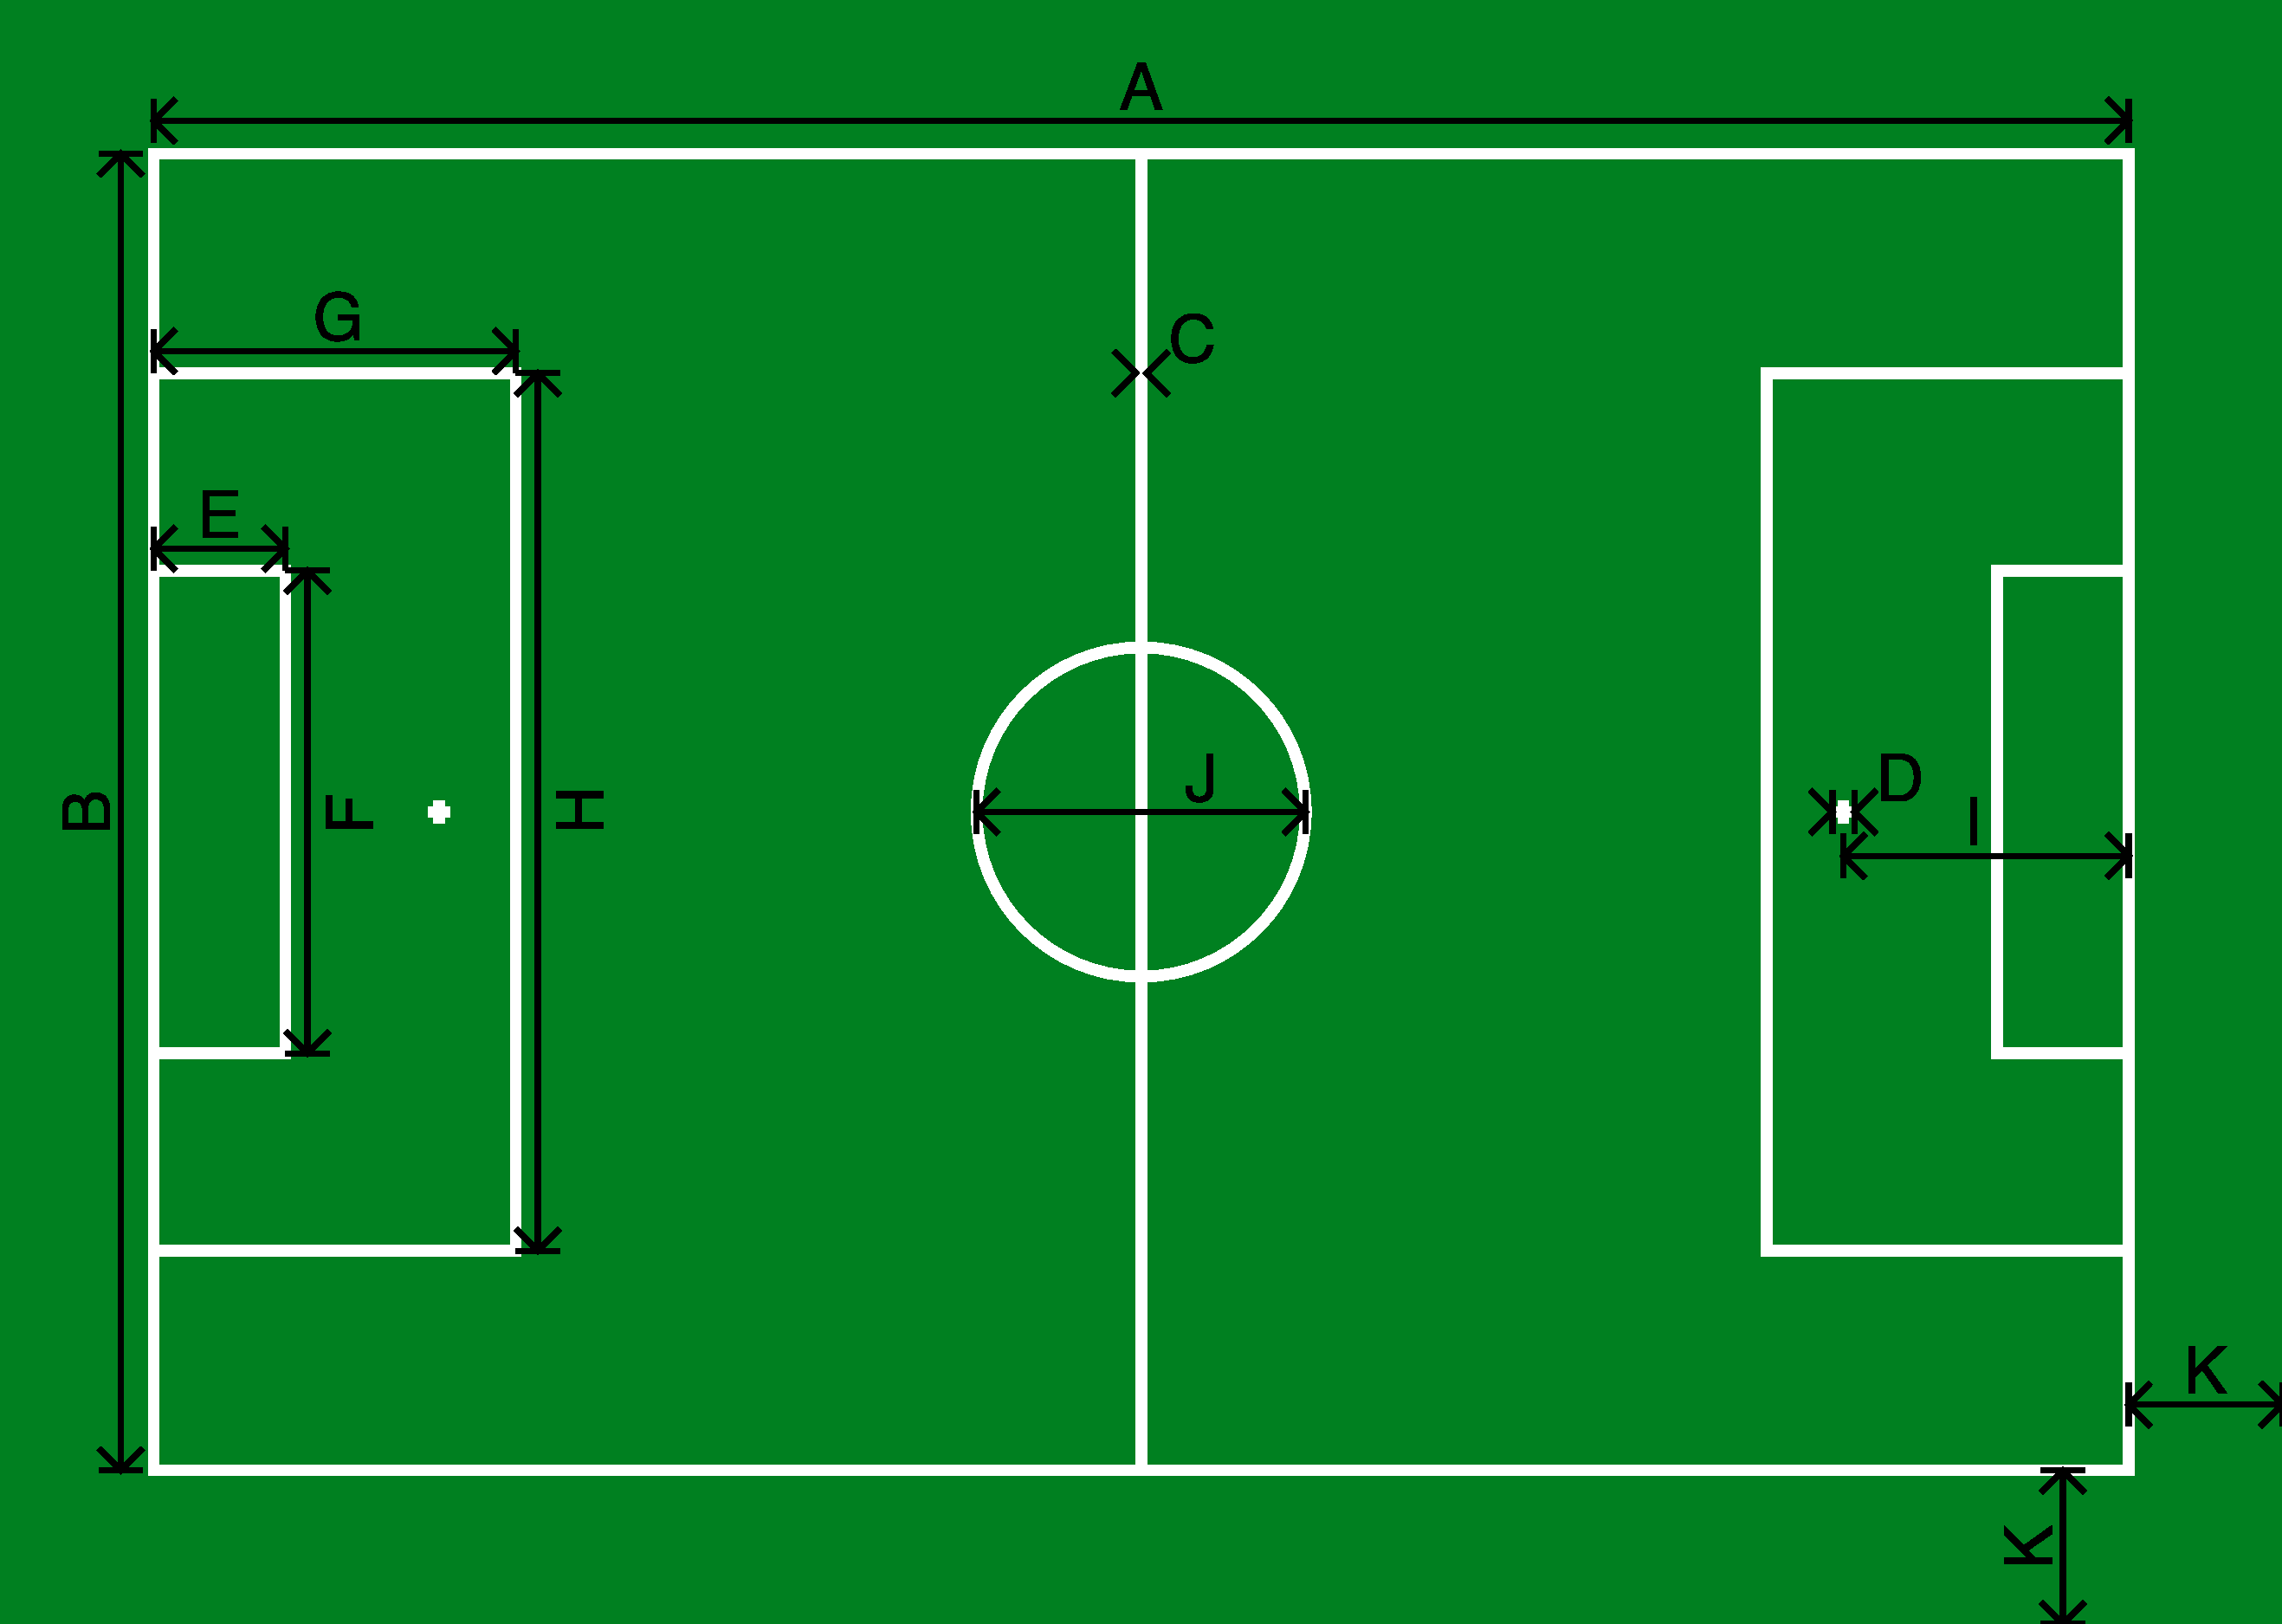
\includegraphics[width=\columnwidth]{figs/fieldDimensions2020.pdf}}
	\vspace{1ex}
	\begin{tabular}{| l | l | l |}
		ID & Description & Length (in mm) \\
		\hline \hline
		A & Field length & 9000 \\
		\hline
		B & Field width & 6000 \\
		\hline
		C & Line width & 50 \\
		\hline
		D & Penalty cross size & 100 \\
		\hline
		E & Goalbox area length & 600 \\
		\hline
		F & Goalbox area width & 2200 \\
	\end{tabular}
	\begin{tabular}{|l|l|l|}
		ID & Description & Length (in mm) \\
		\hline \hline
		G & Penalty area length & 1650 \\
		\hline
		H & Penalty area width & 4000 \\
		\hline
		I & Penalty cross distance & 1300 \\
		\hline
		J & Centre circle diameter & 1500 \\
		\hline
		K & Border strip width & 700 \\
		\hline
		&  &  \\
	\end{tabular}
	\caption{Schematic diagram of the  \cbw{standard} soccer field (not to scale) and corresponding dimensions in mm. Note that measurements on this diagram are made to the centre of lines.} \label{fig:field_dim}
\end{figure}


\begin{figure}[t!]
	\begin{center}
		\leavevmode
		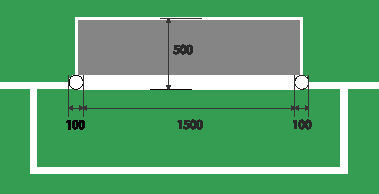
\includegraphics[width=1\columnwidth]{figs/goalDimensions2015.pdf}
		\caption{Dimensions of the goal (in mm), viewed from above, and its placement on the field.}
		\label{fig:goal_dimensions}
	\end{center}
\end{figure}

\begin{figure}[h!]
	\begin{center}
		\leavevmode
		\begin{minipage}[t]{0.49\columnwidth}
			\imagebox{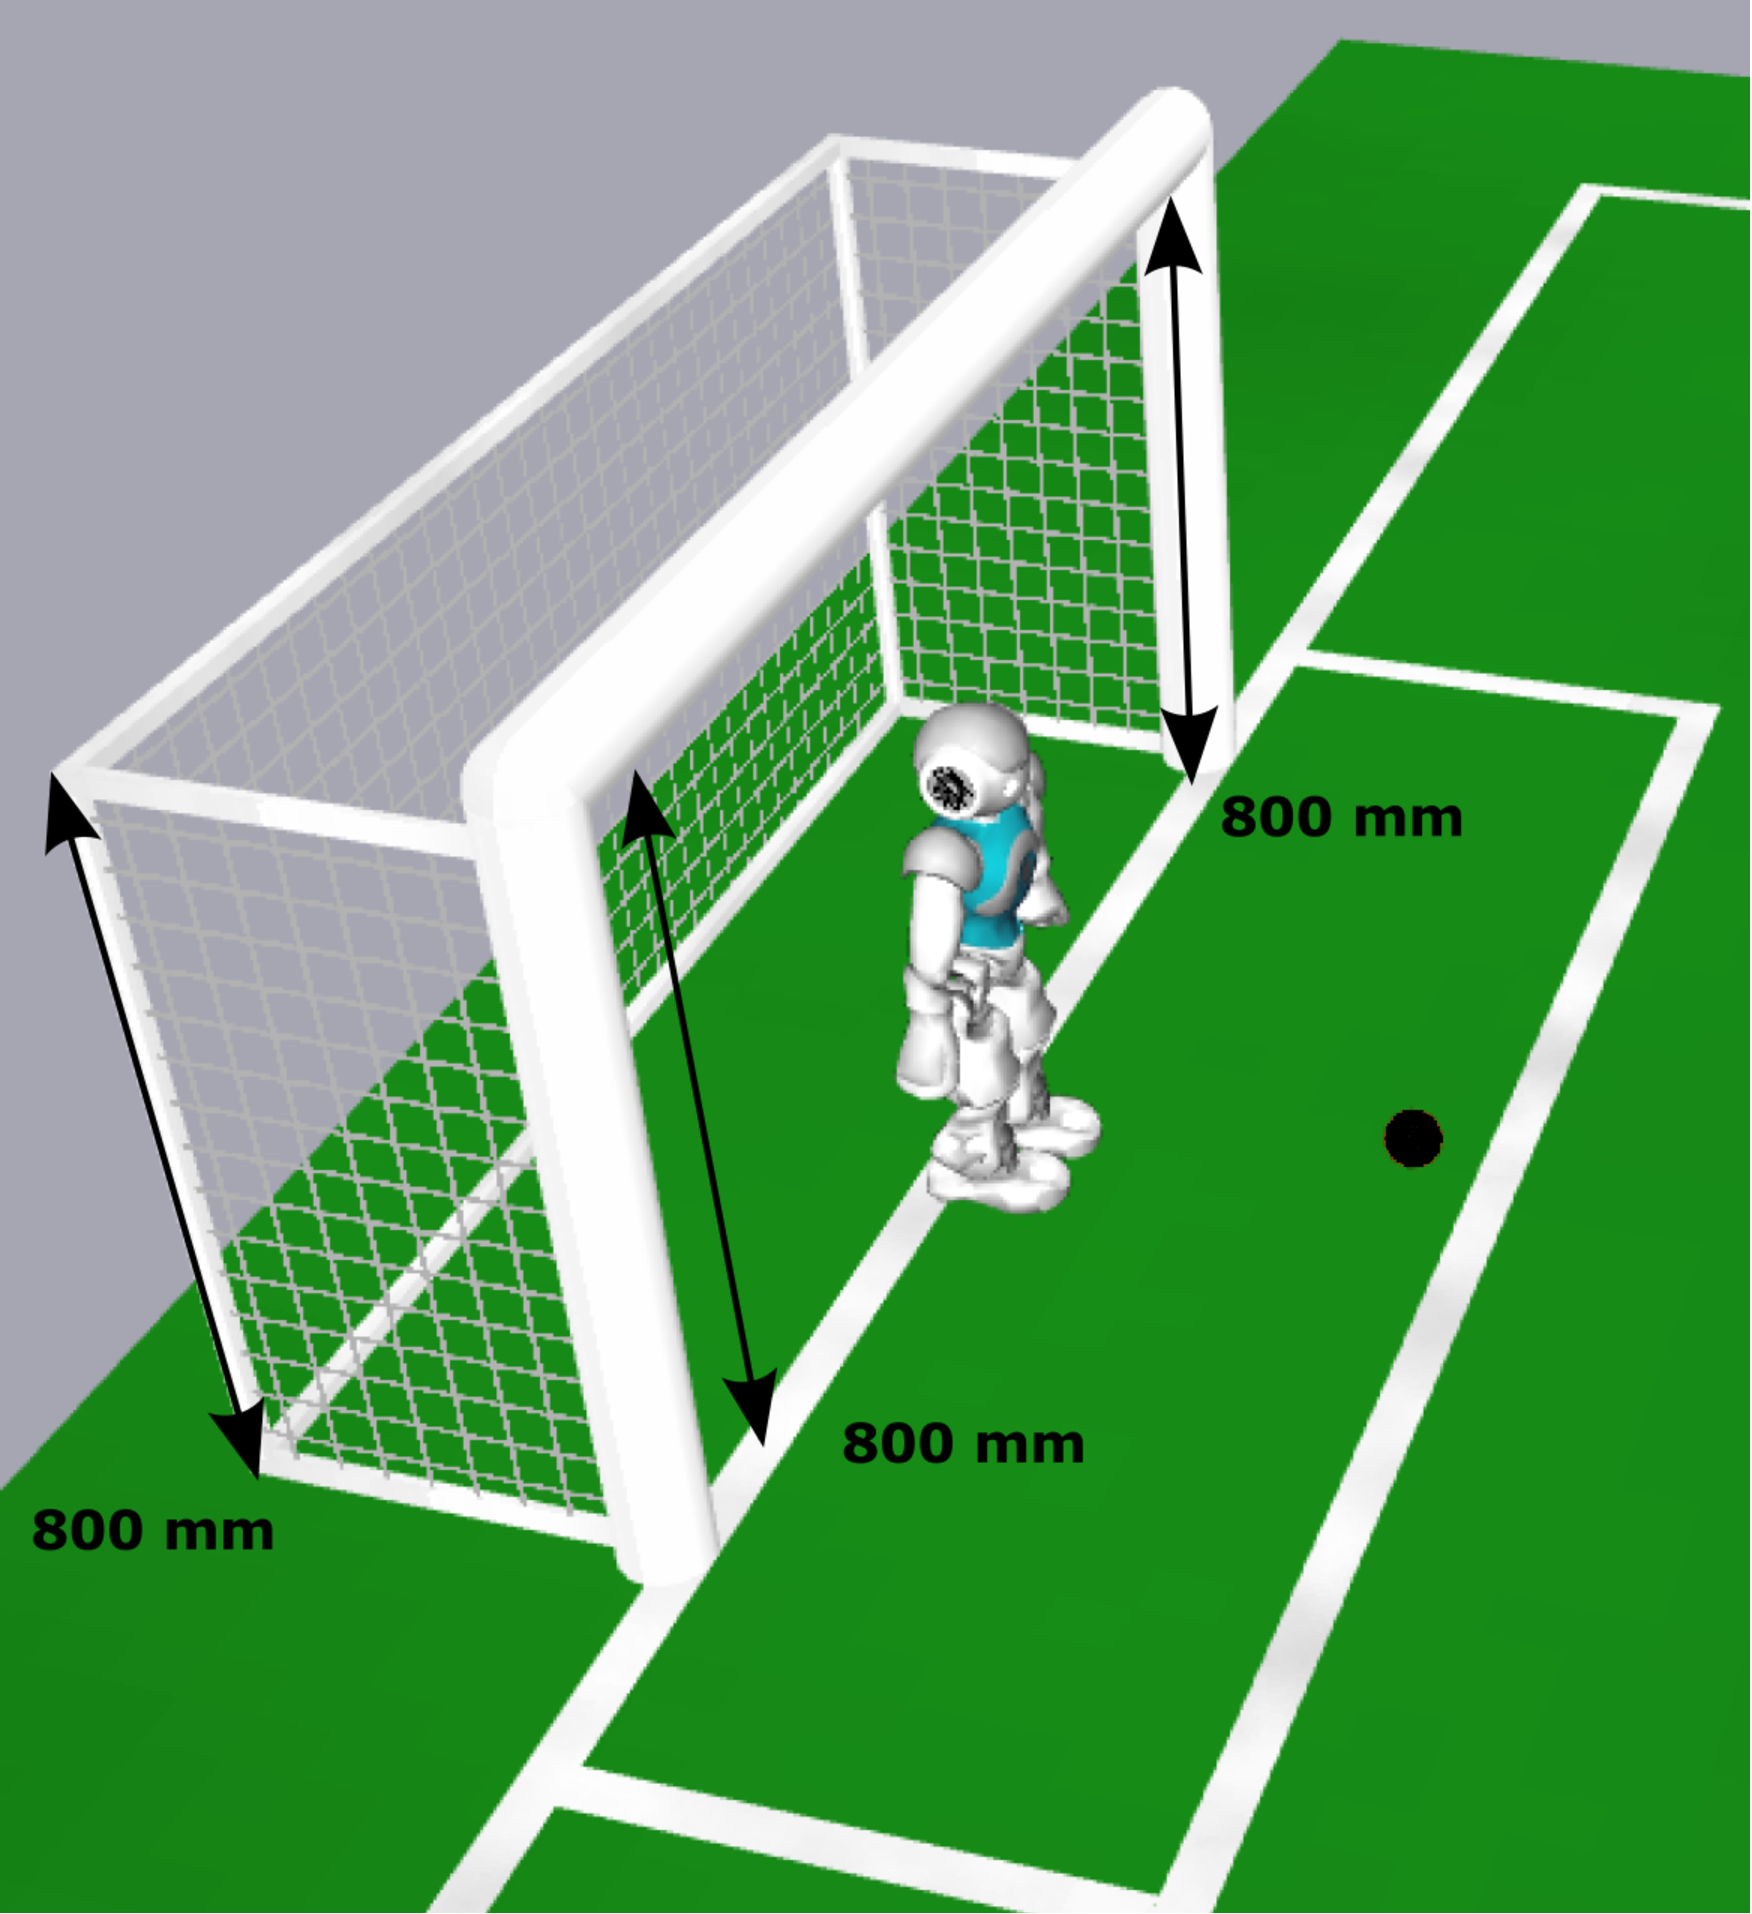
\includegraphics[width=1\columnwidth]{figs/goalDimensions3D.pdf}}%
		\end{minipage}
		\begin{minipage}[t]{0.49\columnwidth}
			The goalposts and crossbar are made from 3 white cylinders with a diameter of 100mm.
			The net:
			\begin{itemize}
				\item has a height of 800mm
				\item is of white, grey or black colour
				\item is tightly supported via the support structure, in a way to minimize interference with the goal keeper
				\item has a weave with holes smaller than the ball diameter.
			\end{itemize}
		\end{minipage}
		\caption{Appearance and dimensions of the goals.}
		\label{fig:goal_appearance}
	\end{center}
\end{figure}

\subsubsection{Field Colours}
\label{sec:field_colors}
The colours of the soccer field are as follow:

\begin{itemize}
	\item The field (artificial turf) itself is green (colour is not specified, but it should not be too dark).
	
	\item The lines on the field are white, whether they are taped, spray painted or made from white artificial turf.
	
	\item Goals~(\cf Figure~\ref{fig:goal_appearance}). The posts and top cross bar of both goals are white. The net and the support structure for the net are white, grey, or black.
\end{itemize}

\subsubsection{Lighting Conditions}
\label{sec:lightConditions}
The lighting conditions depend on the actual \cbw{game venue}. SPL fields \cbw{may} be placed near or under windows where possible. Whether or not window lighting is used, ceiling lights \cbw{should} be provided as necessary to ensure that most of the field is never darker than 300 Lux (400 Lux preferred).

\cbp{Nevertheless, it is not expected that teams should change the lighting setup in their local venue for the purpose of RoboCup 2021.} \\

Lighting is not required to be even and hotspots may occur on the field. The lighting design (comprising both natural and artificial light sources) shall aim to limit the ratio between the brightest and darkest patches on the field to less than 10:1. In general, lighting irregularities, including changes that occur during the competition, are acceptable and will not be cause for delay. Such irregularities may include sun streaming through windows, light bulbs turning off, light bulbs being replaced, etc.

\subsubsection{Ball}
\label{sec:ball}

The official ball is a soft foam ball with a black and white soccer ball print (see Figure~\ref{fig:ball}). They are 100mm in diameter and weigh 44 grams. These balls are available by writing to \url{info@sportpaint.de} (in German or English) and asking to order the "pu schaumstoffball 10cm 100ss".  Each ball costs EUR 2.50 plus shipping, where shipping cost depends on the destination.

\begin{figure}[t]
	\centerline{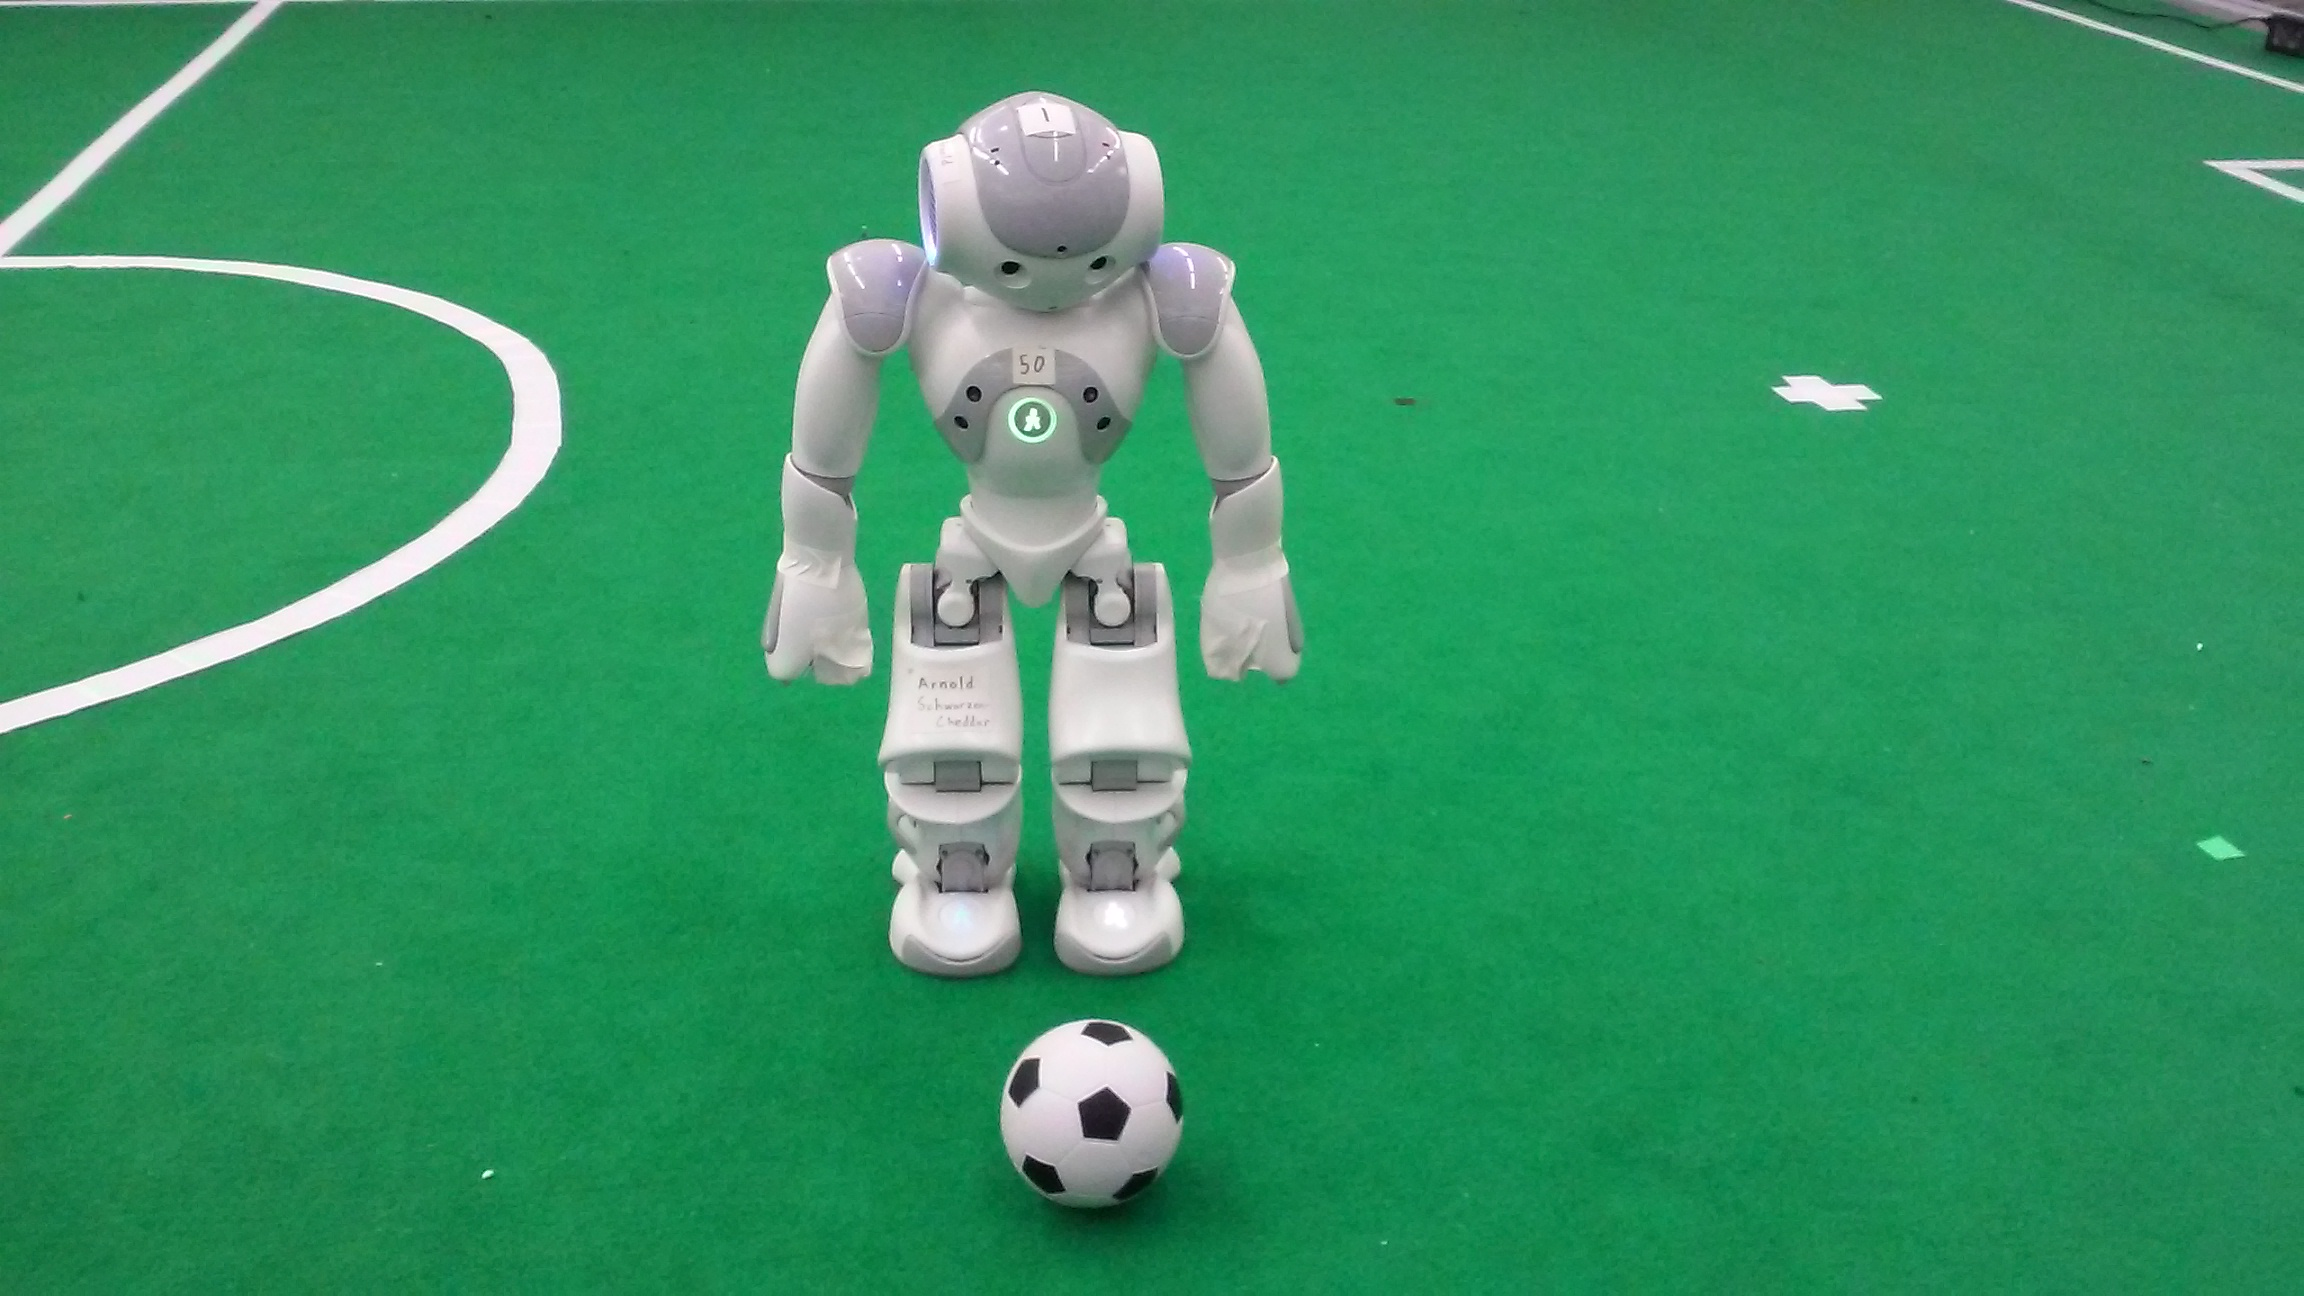
\includegraphics[height=0.28\columnwidth]{figs/robotWithBall2016.jpg}}
	\caption{A NAO and the official ball.}
	\label{fig:ball}
\end{figure}


\subsubsection{Definition of Inside and Outside}
\label{sec:inside_outside}

A line is always part of a region of the field.
This means, that \emph{inside/outside \textless region\textgreater} refers to the green area as well as the surrounding line.
Specifically:
\begin{itemize}
	\item The field boundary lines are part of the field
	\item The penalty box lines (and the end field line inside of the goal) part of the penalty box
	\item The centre circle lines are part of the centre circle
\end{itemize}

The only \textit{exception} to this rule is the centre field line, which does not form part of any half.
That is, a robot is \textit{outside} of a half of the field if it is touching the centre line.

\cbp{\subsection{Challenge streaming setup}
\label{sec:streaming_setup}

There are three use cases for the streaming setup: 
\begin{itemize}
	\item Allow remote referees to judge a remote challenge.
	\item Allow participating teams to watch their robot's challenge
	\item Allow visitors to watch the games and challenges.
\end{itemize}

These cases should be taken into account when setting up a suitable streaming setup with respect to hardware equipment and internet connectivity.
You can think of streaming on YouTube/Discord/BigBlueButton/Zoom ..., whatever is available (If bandwidth in the lab is limited, re-streaming should be considered on system with better network connection). You should consider that referees should get prioritised access to the stream.  
In the root folder of the NextCloud drive (see~\ref{sec:data_exchange}) you find a \texttt{streaming.md} file where every team has to publish a link that can be used by public and teams to watch the challenges and if available another link that can be used by the referees to watch the challenge. The public link will be published on the SPL website / RoboCup 2021 website.}

\subsection{Robot Players}
\label{sec:robot_players}
A match is played by two teams, each consisting of \emph{one player}. All robots are \emph{field players} and no robot is designated as \emph{goalkeeper}.

\subsubsection{Hardware}
\label{sec:hardware}
All teams must use a NAO humanoid robots \cbw{in version 6} manufactured by SoftBank Robotics.

Absolutely no modifications or additions to the robot hardware are allowed. No additional hardware is permitted including off-board sensing or processing systems. Additional sensors besides those originally installed on the robots are likewise not allowed. The only exceptions are:
\begin{itemize}
	\item Setting the passive wrist joints to a fixed position either with glue or a transparent or white duct tape.
	\item Protecting the fingers with white finger protectors provided by the manufacturer or with transparent or white duct tape.
	\item Placing white duct tape over the battery case and screw (under the robot jersey) to keep the battery case in place and prevent the battery becoming disconnected.
	\item A memory stick may remain in the head during operation.  Only ordinary USB flash memory keys that sit flush or recessed to the head casing may be utilized. Other USB dongles or devices, as well as memory sticks that are not flush or recessed, are not permitted.
\end{itemize}

\subsubsection{Field Players}
\label{sec:field_players}
Each field player has a jersey number from the set $\{2, 3, 4, 5, 6\}$. However, by default, \cbw{the number ``2'' is used for the field player}. \cbw{This assignment can be changed due to availability of jerseys.}

\cbp{\subsubsection{Stationary Obstacle Robots}
\label{sec:stationary_obstacle_robots}
Some of the challenges use stationary obstacle robots. \\
	
All stationary obstacle robots are allowed to stand upright or sit down and can remain turned off for the duration of the challenge. Static obstacle robots may not lay down on the field. Stationary obstacle robots are not required to be V6 edition NAO robots. It is allowed to use any NAO edition that was legal to use in a RoboCup SPL competition in the past. \\

Stationary obstacle robots are required to not wear any jerseys.}


\subsubsection{Team Markers}
\label{sec:team_markers}
Robots use coloured jersey shirts as team markers in the ``home'' and ``away'' colours of the hosting arena team. Each jersey shirt has a player number (1-6) printed on it. \cbw{The use of player number 1 is disallowed in the challenges of the 2021 competition.} The team markers are worn as shown in Figure~\ref{fig:nao_markers}.

\begin{figure}
	\centerline{\begin{tabular}{lll}
			a) & b) & c) \\
			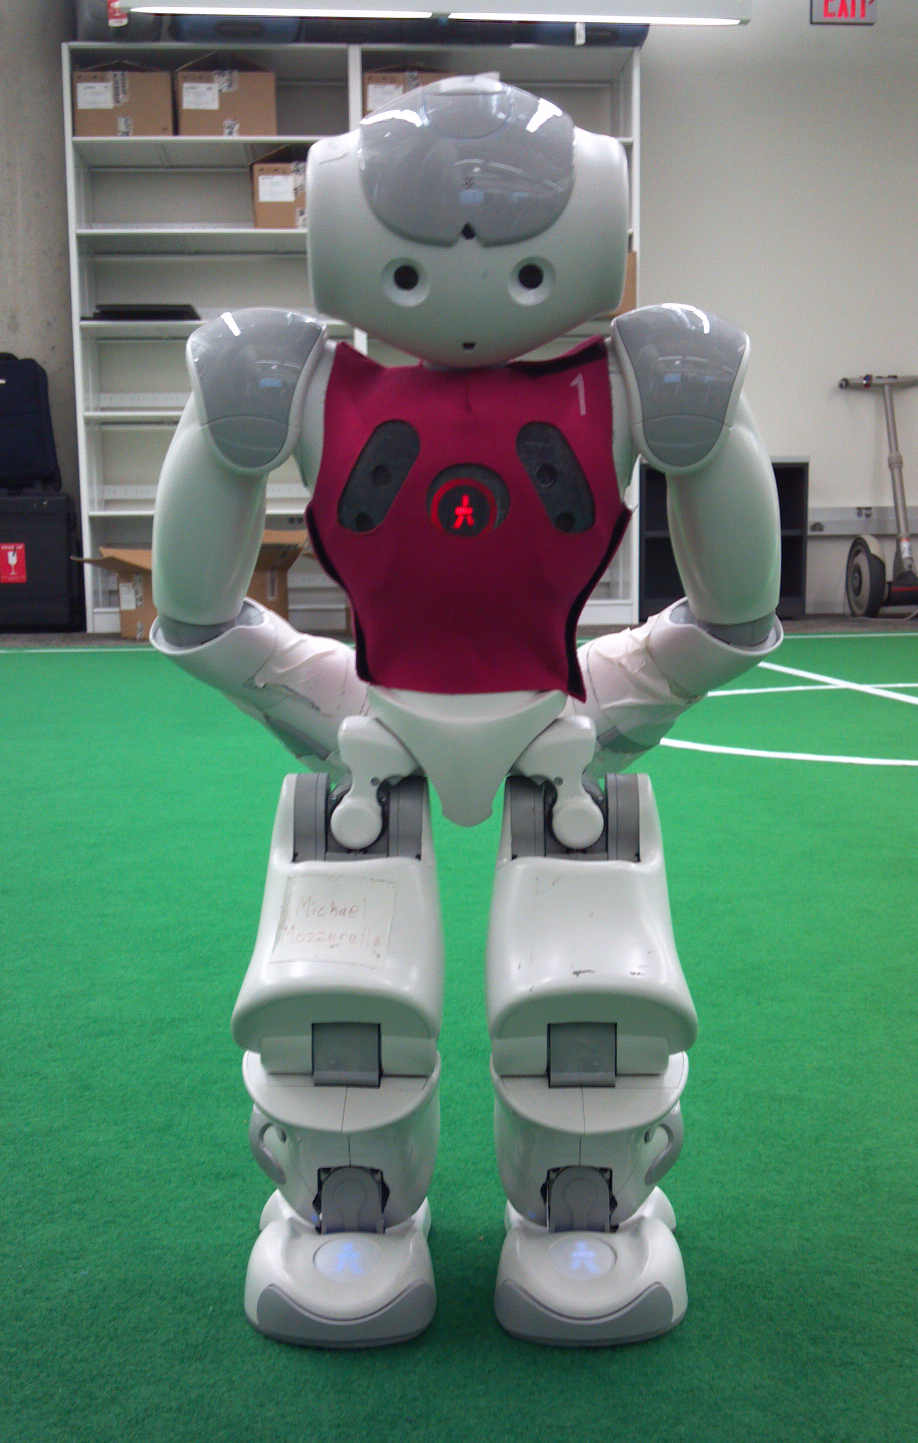
\includegraphics[height=0.28\columnwidth]{figs/front.jpg}&
			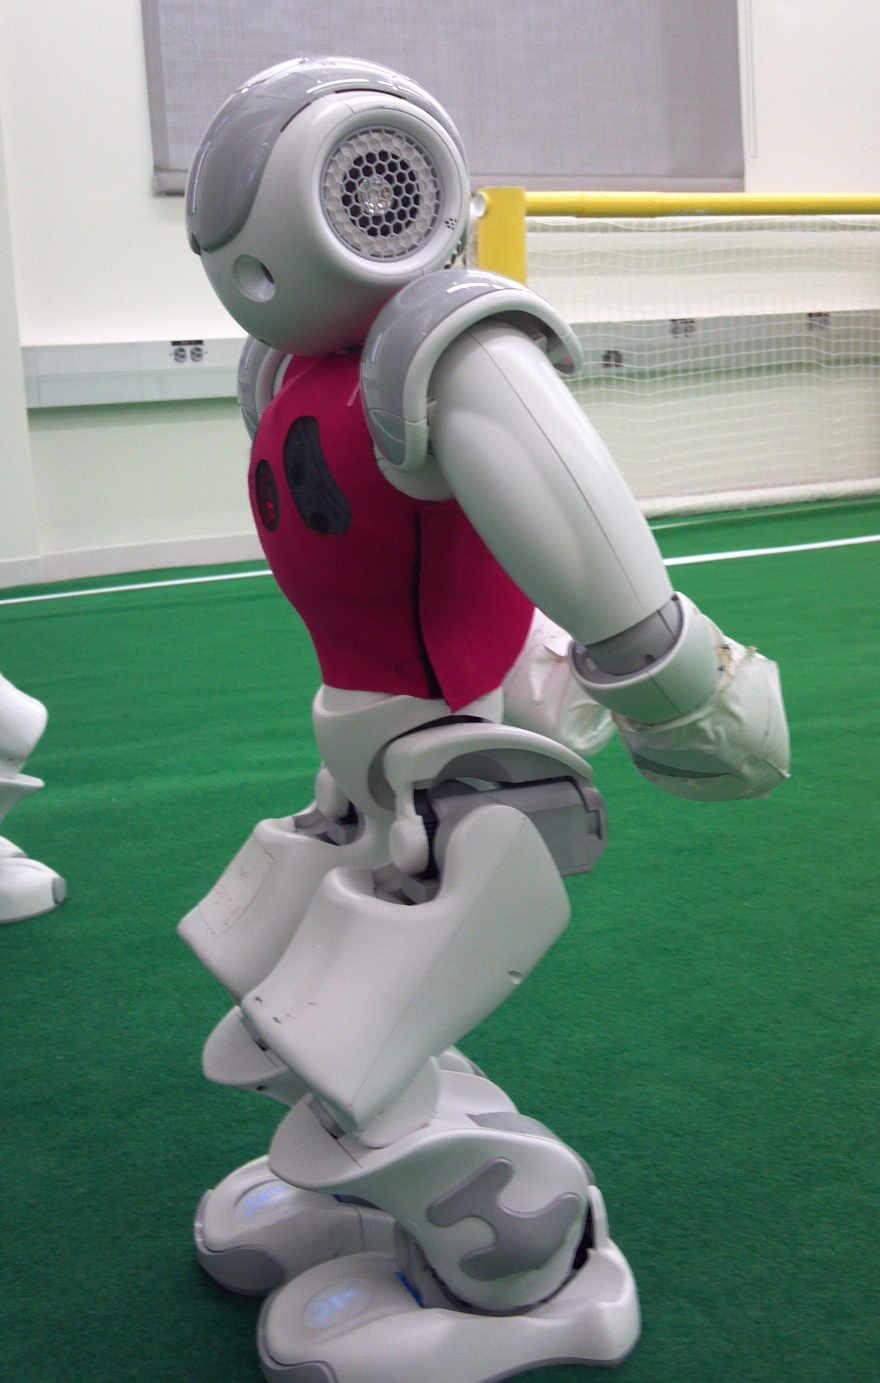
\includegraphics[height=0.28\columnwidth]{figs/side.jpg} &
			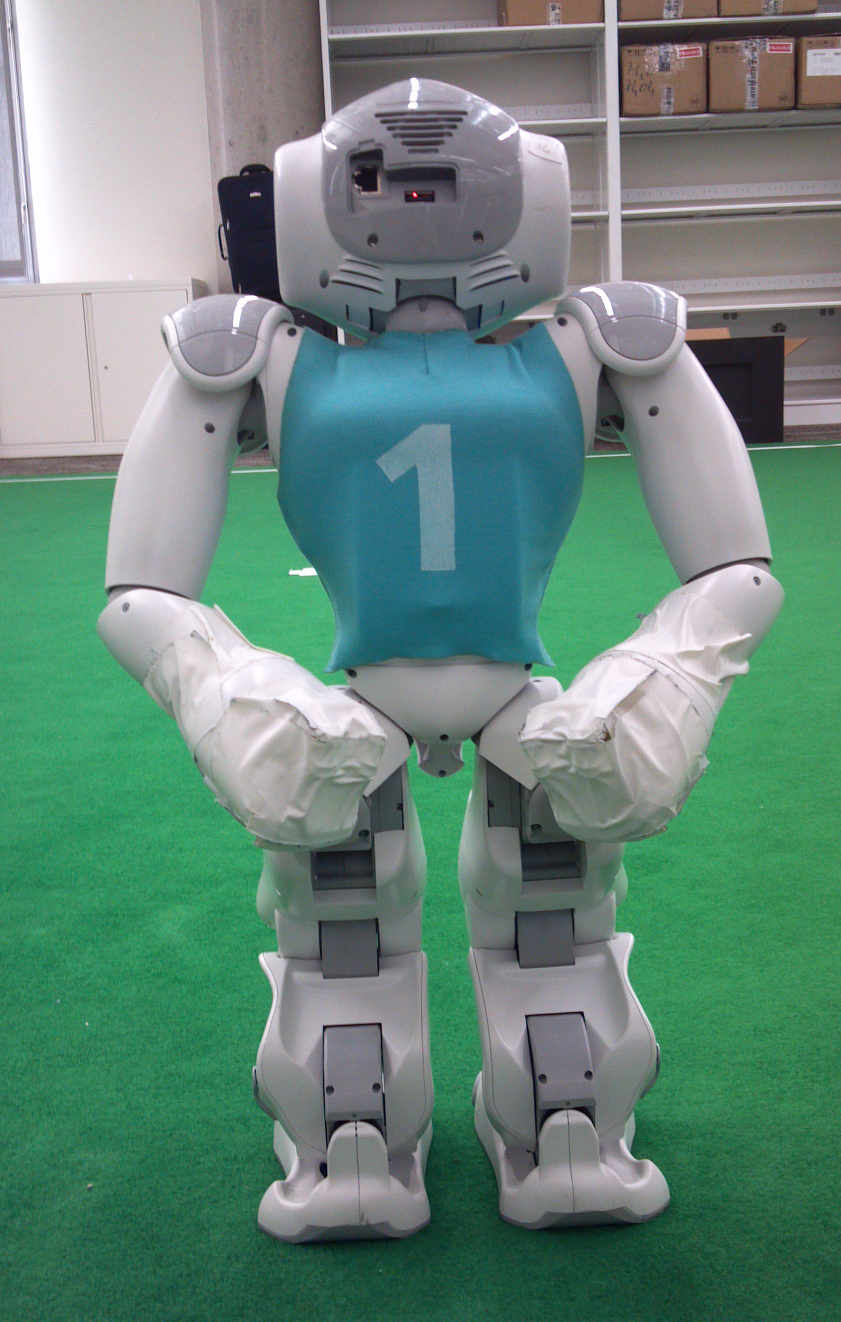
\includegraphics[height=0.28\columnwidth]{figs/back.jpg}
	\end{tabular} }
	\caption{Team markers. a) Front view. b) Side view. c) Back view.}
	\label{fig:nao_markers}
\end{figure}
\cbp{Teams may use any jersey that was approved for a RoboCup SPL competition in the last 4 years without needing to reapprove it in 2021.}

Teams may design and manufacture their own jerseys in any colour (multi and many colour jerseys are acceptable), but must follow these guidelines:
\begin{itemize}
	\item Jerseys should be the tank top style used at RoboCup 2013/2014 and should cover approximately the same areas of the robot as shown in Figure~\ref{fig:nao_markers}.  The torso LED must be clearly visible.  Jerseys may include the sonar panel used in the 2013/2014 jerseys, although this is not required.
	\item Jerseys must have a primary colour that comprises at least 70\% of the jersey.
	\item Jerseys should not contain distractors, such as large pictures of SPL balls or white stripes on green jerseys.
	\item All players on a team must wear identical jerseys.
	\item A team must wear the jerseys that it starts a game in for the entire game.
	\item Jersey material must be non-reflecting, non-shiny, and non-textured.  Material that is glittery is also not appropriate.
	\item Jerseys should be numbered 1-6 on both sides. The numbers must be large and {\bf easily} recognized by humans. \cbw{The use of player number 1 is disallowed in the challenges of the 2021 competition.}
	\item Teams must have two sets of jerseys that are significantly different in terms of their primary colour.
	\item Designs must be submitted to \url{rc-spl-tc@lists.robocup.org} for approval by May 1st, 2021. If the team has jersey prototypes, they should submit close-up images of a robot wearing the jersey - these images should be taken from front, back, and side angles.  If the team has no prototypes, then designs depicting the expected jersey should be submitted.  If submissions show separated front and back halves of jerseys then the team must specify which halves are matched to form home and away jerseys.  All images and designs should be submitted in pdf or jpg format.
\end{itemize}

Each team/arena must designate a ``home'' colour and an ``away'' colour when asked about one month before RoboCup. Robots must wear the `home' jerseys when they are ``home'' (the first team listed on the schedule). The ``away'' team (the second team listed on the schedule) will wear the ``away'' jerseys.

Some teams wish to include additional information or logos on their robots. The following are allowable:
\begin{itemize}
	\item Attaching player numbers to the heads and/or legs of the robots.  These numbers should be black with a white background, and should correspond to the number on the robot's jersey.
	
	\item Adding sponsor or team logos to the upper legs of the robots (\cf Figure~\ref{fig:sponsor}). A box drawn around the non-white area of these logos must not cover more than a 25 $\text{cm}^2$ area. At most one logo may be attached per leg --- if you wish to attach more than one logo per leg, email the Technical Committee at least two weeks before the competition.  Depending on the size and design of the logos, this may be allowable.
	
	\item Adding small black and white stickers to the torso of the robots stating the name of the robot, the name of the team, or similar information. These stickers must be small and mostly white.
\end{itemize}

\begin{figure}[b]
	\centerline{\begin{tabular}{ll}
			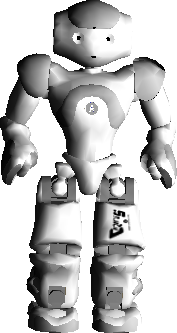
\includegraphics[height=0.35\columnwidth]{figs/naosim_with_logo.png}&
			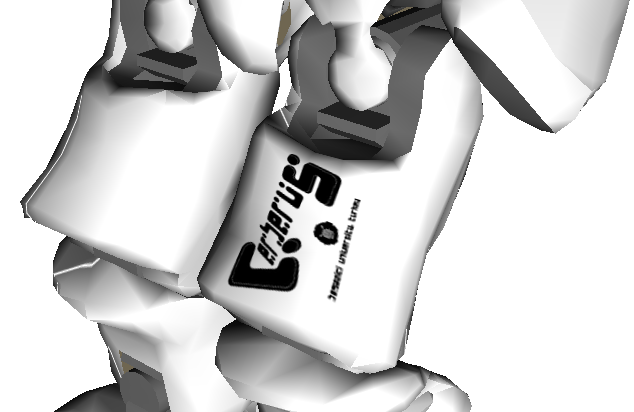
\includegraphics[height=0.35\columnwidth]{figs/naosim_legs_with_logo_closeup.png}
	\end{tabular}}
	\caption{Example Sponsor/Team Logo placement on legs.}
	\label{fig:sponsor}
\end{figure}

\subsubsection{Wireless Communications}
\label{sec:wireless}
The robots must play without human control. Communication is only allowed between a robot and the GameController.

The only wireless hardware allowed to be used by the teams/arenas are the wireless network cards built into the NAOs, and the access points provided by the arena. All other wireless hardware must be deactivated. A team/arena may be disqualified if one of the team members violates this rule.

Each team will get a range of IP addresses that can be used both for their robots and their computers/remote connections. The network configuration (\eg IP addresses, channels, SSIDs, and required encryption) of the fields \cbw{will be announced (\cf Section~\ref{sec:c3_BasicRequirementsForArenas})}.

Teams and their robots must not listen into another team's communication.

The GameController will use UDP to connect to the robots. The source distribution of the GameController provides the header file \emph{RoboCupGameControlData.h} that defines all messages sent by the GameController to the robots. They correspond to the \emph{robot states} described in Section~\ref{sec:robot_states}.

Robots send status updates (defined in \emph{RoboCupGameControlData.h}) to the GameController. These return packets must be addressed directly to the GameController PC (\ie not broadcast) and sent on the GameController return UDP port specified by the symbol \verb!GAMECONTROLLER_RETURN_PORT! in \emph{RoboCupGameControlData.h}.

The use of remote processing/sensing is prohibited.

\subsection{Game Process}
\label{sec:game_process}

\subsubsection{Structure of the Competition}
\label{sec:game_struct}

\cbp{Unless otherwise specified, a competition consists of three parts, the first half, a half-time break, and the second half. Each half is 5 minutes counted from the initial kick-off.} \\
	
\cbp{The half-time break is five minutes and code changes are prohibited in the half-time! It is mainly used to cool down the robots and to charge them.}

The head referee signals the commencement of each half with a single whistle blow (that is, the Initial kick-off, \cf Section~\ref{sec:initial-kick-off}).
The head referee signals the end of the first half with two short whistle blows, and the end of the second half with two short plus one long whistle blow.
The head referee should make \textit{all} of these whistle sounds from the T-junction of the half-way line.

The teams/robots will change the goal defended during the half-time break.

\subsubsection{Robot States}
\label{sec:robot_states}

Robots can be in \textit{eight} different \emph{primary} states (\cf Figure~\ref{fig:robot_states}). \cbw{Wireless connection must be available}, so these states will be set by the GameController. Teams must implement code to receive and correctly respond to wireless GameController packets, and also give a visual indication of the game state.

\cbp{\textbf{The use of the button interface as a replacement for any GameController commands is not allowed in the 1vs1 competition!}}

\cbp{Should both robots have problems with the Wifi/GameController connection the head referee should issue a referee timeout (\cf Section~\ref{sec:referee_timeout}).}
If \cbw{only one} robot does not respond to the GameController then it is not included in the game (via a `Request for Pick-up', \cbw{\cf Section~\ref{sec:request_for_pickup}}), and the game starts without the offending robot.

\begin{description}
	\item[Initial.] After booting, the robots are in their \emph{initial} state. The robots are not allowed to be moving in any fashion besides initially standing up. Shortly pressing the chest button will switch the robot to the \emph{penalized} state.
	
	\item[Ready.] In this state, the robots walk to \cbw{a legal position on their half}. They remain in this state, until the head referee decides that there is no significant progress, up to a maximum of \KickOffAutoTime.
	
	\item[Set.] In this state, the robots stop and wait for Kick-Off  (\cf Section~\ref{sec:kick-off}).
	Illegally positioned robots are penalized.
	Robots are allowed to move their heads or get up if fallen before the game (re)starts but they are not otherwise allowed to move their legs or locomote in any fashion.
	If a robot cannot get up, fallen robot is called~(\cf Section~\ref{sec:fallenrobots}).
	The penalty time counter is frozen during this state.
	Note that all penalized robots are left in place (on the side of the field, or in-place for motion in set) and must wait to get unpenalized.
	
	\item[Playing.] In the \emph{playing} state, the robots are playing the competition. Shortly pressing the chest button will switch the robot to the \emph{penalized} state.
	
	\item[Penalized.] A robot is in this state when it has been penalized. It is not allowed to move in any fashion,  this includes stopping the head turning. Shortly pressing the chest button will switch the robot back to the \emph{playing} state.
	
	\item[Finished.] This state is reached when a half is finished.

	\item[Unstiff.] \cbw{\textit{This state has been added in 2021.}} It helps to facilitate a consistent and safe handling of the robots for remote competition. During any states, if all head buttons are pressed for at least one second by the referees, the robot should move to a safe seated/crouched position and unstiffen all joints. Pressing all three head button while in the Unstiffen state for at least one second by the referees, permits the robot to stiffen it's joints and return to the initial state, or a state as indicated by the GameController.

	\item[Calibration.] \cbw{\textit{This state has been added in 2021.}} This state denotes the robot is acting with automatic calibration. This state may only be entered from Initial by first pressing the \textit{front} head button concluded by the chest button, for at least one second by the referees.
    
\end{description}

\begin{figure}[t]
	\centerline{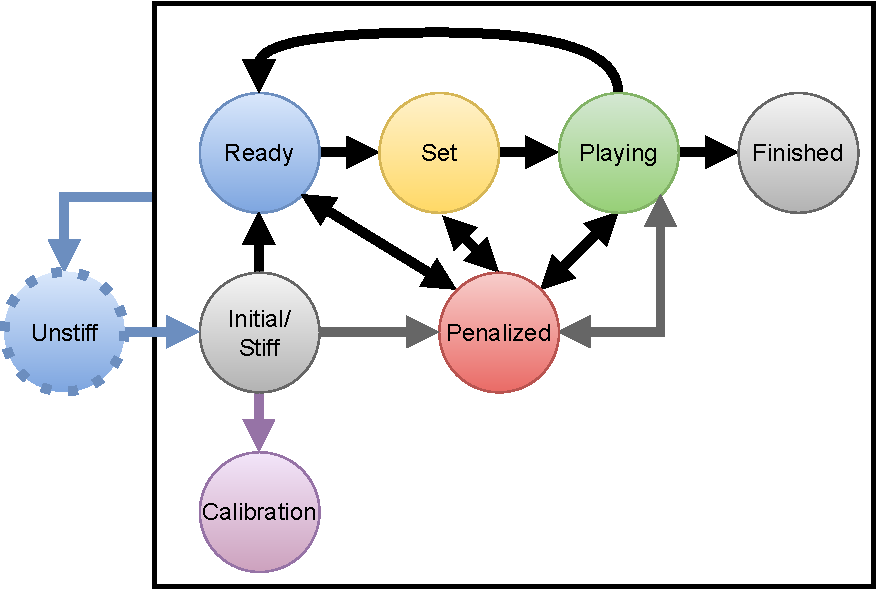
\includegraphics[width=0.9\columnwidth]{figs/states_new.pdf}}
	\caption{\cbf{Diagram of the robot states. 
    \\\textbf{Chest button} transitions are shown as grey arrows. However, any transition possible should be sent by the GameController.
    \\\textbf{GameController} transitions are shown as black arrows. 
    \\Calibration transitions are shown as puple arrows which mean pressing the \textbf{front head button + the chest button}.
    \\From any state it can be transitioned to the \textit{unstiff} state, shown as a blue arrow, via pressing all \textbf{three head buttons}. Pressing all \textbf{three head buttons} in the \textit{unstiff} state allows a transition to the initial state, or a state as indicated by the GameController}}
	\label{fig:robot_states}
\end{figure}

The referee will announce the start of the Playing state with a single whistle blow.
The GameController Playing signal will be delayed by \PlayingDelayTime.
Robots that begin moving their legs or locomoting in any fashion during \emph{set} (\ie before the referee blows the whistle) will be penalized \textit{in place} on the field via the ``Motion in Set'' (\cf Section~\ref{sec:motion_in_set}) GameController signal (and moved back to their original position if they have moved significantly before becoming penalized) until the GameController transmits the \emph{Playing signal}.

The current game state should be displayed on the LED in the torso. The colours corresponding to the game states are:

\begin{itemize}
	
	\item Initial: Off
	
	\item Ready: Blue
	
	\item Set: Yellow
	
	\item Playing: Green
	
	\item Penalized: Red
	
	\item Finished: Off
	
    \item \cbw{Unstiff: Blue-Blinking - \textit{optional}}

    \item \cbw{Calibration: Purple - \textit{optional}}
\end{itemize}

The current GameController requires robots to know both their team number and their robot number within the team. It is each team's responsibility to make sure this is correctly configured. It is recommended that the robot indicates its number within the team on boot-up so that this can be easily checked at the start of the game.

\subsubsection{Goal}
\label{sec:goal}
A goal \cbw{(including own goal)} is achieved when the entire ball (not only the centre of the ball) goes over the goal-side edge of the goal line, \ie the ball is completely inside the goal area\footnote{The goal line is part of the field.}.

\cbp{If any robot player scores a goal (including own goals) the ball gets replaced by the referees to one of the ball starting points in the scoring teams half of the field. Note that for an own goal the ball is placed on the opponents half and is a disadvantage in two senses. The ball is placed on the ball starting point farthest away from the player in this half (unless blocked by a ball then the other goalbox corner is used). If the two corners of the goalbox are occupied, the two corners of the penaltybox are used, starting with the one farthest away from the robot. The ball can be played again without delay.}

The head referee signals a goal by a single whistle blow, followed by the call ``Goal \textless colour\textgreater''. \cbp{However no GameController action shall be performed.}

%TODO: Maybe we can change the logic of the GameController to allow for counting goals without ready and set phase.
\cbp{After the game is in the state playing, the game state remains in it regardless of shot goals or scored points! Exceptions are the application of the Global Game Stuck rule and a referee timeout, \cf Section~\ref{sec:game_stuck:global} and Section~\ref{sec:referee_timeout}}


\subsubsection{Initial Kick-off}
\label{sec:initial-kick-off}

The first kick-off at the start of each half is the initial kick-off.
Before the initial kick-off, \ie before the start of each half, \cbw{both} robots must be in the initial state and must be placed on the sidelines, \cbw{closest to the GameController}, in their own half of the field \cbw{at the height of the penalty spot}. 
Once the robots receive the \emph{ready} signal from the GameController, they are to proceed as described in Section~\ref{sec:kick-off}.

\subsubsection{Kick-off}
\label{sec:kick-off}
For kick-off, the robots listening to the wireless GameController run through three states: \emph{ready}, \emph{set}, and \emph{playing}. \cbw{It is to a team's responsibility to have their robots listen to the GameController!}

In the ready state, the robots should walk to their legal kick-off positions.
\cbp{The players can be positioned anywhere within their own half, but no player is allowed to touch the centre / halfway line.} 
All robots that do not reach legal positions will be penalized with the ``Illegal Position'' penalty~(\cf Section~\ref{sec:illegal_positioning}).

In the \emph{set} state, the robots must not locomote~(\cf Section~\ref{sec:robot_states}). A referee places \cbw{the two balls, for each side, on the goal free kick positions (\cf Section~\ref{sec:kick_in}).}
If the ball is moved by one of the robots during \emph{set} it is replaced by one of the referees.

\cbp{There is no manual placement of any robot.}

The head referee signals the kick-off by a single whistle blow, followed by the call ``Playing''. The head referee must signal this from the T-junction of the half-way line.

After the head referee has signalled the kick-off, the robot's state is switched to \emph{playing} by the GameController.

\subsubsection{Kick-in}
\label{sec:kick_in}

A ball is considered to have left the field when there is no part of the ball over the outside of the boundary line (\ie the line itself is in). \\
\cbp{If the ball goes over a sideline then the assistant referee will replace the ball back on the point of that sideline where it went out.} \\
\cbp{If the ball goes over an end-line then the assistant referee will replace the ball onto the corner of the goal box on the same side of the field that the ball was kicked-out. That is, the corner inside the field, not the t-junction where the goal box meets the goal line. If the corner is blocked by a robot or ball then the other goalbox corner is used.}
\cbp{Note that no GameController action is required.}

\subsubsection{Global Game Stuck}
\label{sec:game_stuck:global}

In the event of no ``substantial change''\footnote{``substantial change'' can consist of a robot seeing and moving towards the ball OR robots exploring the field (presumably in an attempt to find the ball)} in the game state for 30 seconds OR \cbw{no ball was played from one half to the other for more than 1 minute}, this is considered a global game stuck and the referee calls ``Global Game Stuck''. 

\cbp{Once the referee calls Global Game Stuck, players enter the Ready state and a new kick-off (\cf Section~\ref{sec:kick-off}) is awarded.}
%TODO: Single GameController button for Global Game Stuck?
%TODO: Global game stuck starts with Initial position


\subsubsection{Request for Pick-up}
\label{sec:request_for_pickup}

Either team may request that their players be picked up (called ``Request for Pick-up'').
In the Playing or Ready state, players may only be picked up for hardware failures.
In all other states, players may be picked up for any reason.

\cbp{Only hardware changes are allowed during a request for pick-up! In particular, it is permitted to change batteries, fix mechanical problems, reboot the robots. Since the teams are not on site, the assistant referees take over these tasks as if they were a member of the corresponding team.}

\cbp{However it is prohibited to change the robot's control program or any configuration file.}

Any strategic ``Request for Pick-up'' is not allowed.
That is, gaining an advantage by removing the robot from the competition.
In this case, the head referee will indicate when the robot is no longer affecting play and can be removed from the field by an assistant referee.

To prevent mistakes and confusion during games, only team leaders should make a ``Request for Pick-up''.

The returning robot may be returned following the normal replacement procedure once at least 45 seconds have elapsed since the robot was removed from play. Note that this penalty does not follow the standard removal procedure, and hence does not count towards the incremental penalty count.

If the picked-up robot was penalized, the penalty time of the robot counts down with the game clock throughout the pick-up.
Note here, that the returning robot will have to wait out any remaining penalty time of the picked up robot after the team handed their robot back to the assistant referees.

\subsubsection{Referee Timeout}
\label{sec:referee_timeout}
The head official may call a timeout at any stoppage of play if he or she deems it necessary. A referee timeout should only be called in dire circumstances --- one example might be when the power to the wireless router is down \cbw{or no robot listens to the GameController}. However, when and whether to call a referee timeout is left up to the head referee.

Referees may call multiple timeouts during a game if needed. Teams are \cbw{only allowed to do hardware changes} during these timeouts and they must be ready to play \textbf{2 minutes} after the referee ends a timeout. The referee should end the timeout once he or she believes the circumstance for which the timeout was called has been resolved. In cases where the circumstance for which the timeout was called is not resolved within 10 minutes, the chair of the technical committee should be consulted regarding when/if play should continue.

\subsection{Forbidden Actions and Penalties}
\label{sec:forbidden_act}

The following actions are forbidden. In general, when a penalty applies, the robot shall be replaced, not the ball.

\cbp{Since teams are playing with robots from other teams, there is a maximum of 3 hardware related penalties:
\begin{itemize}
	\item \textbf{fallen robot} or \textbf{inactive robot}, \cf Section~\ref{sec:fallenrobots}
	\item \textbf{request for pick-up} in the Playing or Ready state - either by the team or by the head referee, \cf Section~\ref{sec:request_for_pickup} and Section~\ref{sec:damage_robot}
	\item Robots are not allowed to dive for the ball on purpose, \cf section \ref{sec:fallenrobots}.
\end{itemize}
After that this robot is excluded for the rest of the competition!}

\cbp{If it comes to an excluding of a robot, the head referee, in consultation with the two team leaders, must decide whether the hardware errors that occurred were exclusively self-inflicted due to faulty code or whether it was a general hardware problem with the robot.}\\

\cbp{Depending on this decision:
\begin{itemize}
	\item In case of self-inflicted hardware problems will the game continue without this robot till the end of the regular time or till the remaining robot scores more points or stop if it has more points scored than the excluded robot. 
	\item For general hardware-related errors of the robot, it will be replaced by another robot and the game will be restarted as soon as possible which depends on how much time this team needs to flash, setup and recalibrate the robot. This must not take longer than the official time for a remote setup (\cf Section~\ref{sec:remote_game_setup})!
\end{itemize}}

\cbp{A robot exchange can take place at most once per team, in this case this competition would be restarted 2 times!}

%TODO: Right spot?

\subsubsection{Penalty Procedure}
\label{sec:penalty_procedure}

When a robot commits \cbw{an infraction}, the head referee shall call out the infraction committed, the primary jersey colour of the robot, and the jersey number of the robot. The penalty for the infraction will be applied immediately by an assistant referee. The assistant referees should perform the actual movement of the robots for the penalty so that the head referee can continue focusing on the game. The operator of the GameController will send the appropriate signal to the robots indicating the infraction committed.

For penalties that are timed, the penalty time is considered to be over at the end of each half.

\subsubsection{Standard Removal Penalty}
\label{sec:removal_penalty}

Unless otherwise stated, all infractions result in the removal of the infringing robot from the field of play for a particular amount of time, after which it will be returned to the field of play. This process is called the \textit{standard removal penalty}.

When the head referee indicates \cbw{an infraction} has been committed that results in the standard removal penalty, the assistant referee closest to the robot will remove the robot immediately from the field of play. The robot should be removed in such a way as to minimize the movement of other robots and the ball. If the ball is inadvertently moved when removing the robot, the ball should be replaced to the position it was in when the robot was removed.

The GameController will send the appropriate penalty signal to the robot indicating the infraction committed. After a penalty is signalled to the robot, it is not allowed to move in any fashion. The removed robot will be placed outside of the field facing away from the field of play.

The initial duration of the standard removal penalty time is \StandardPenaltyTime.
Unless otherwise specified, the penalty time increases by \StandardPenaltyIncrease each time a team commits any infraction.
That is, the first infraction will result in a penalty time of \StandardPenaltyTime, the second infraction (of any type) results in a penalty time of 55 seconds, the third infraction is 65 seconds, etc.

During the \emph{set} state the penalty time counter will not decrease.

The GameController will keep track of the time of the penalty. The operator of the GameController will signal the assistant referees when the penalty is 10 seconds from being over, so that one of them can place the robot in the half of the field which this robot's team is defending and \cbw{on the sideline that is nearest to the GameController}. The robot should be placed close to the position where the penalty spot projects on the sideline. This is illustrated in Figure~\ref{fig:penalty_re-entry_points}.

With approximately 5 seconds left before the penalty ends, the robot should be turned to face towards the opposite sideline.

\begin{figure}[t]
	\centerline{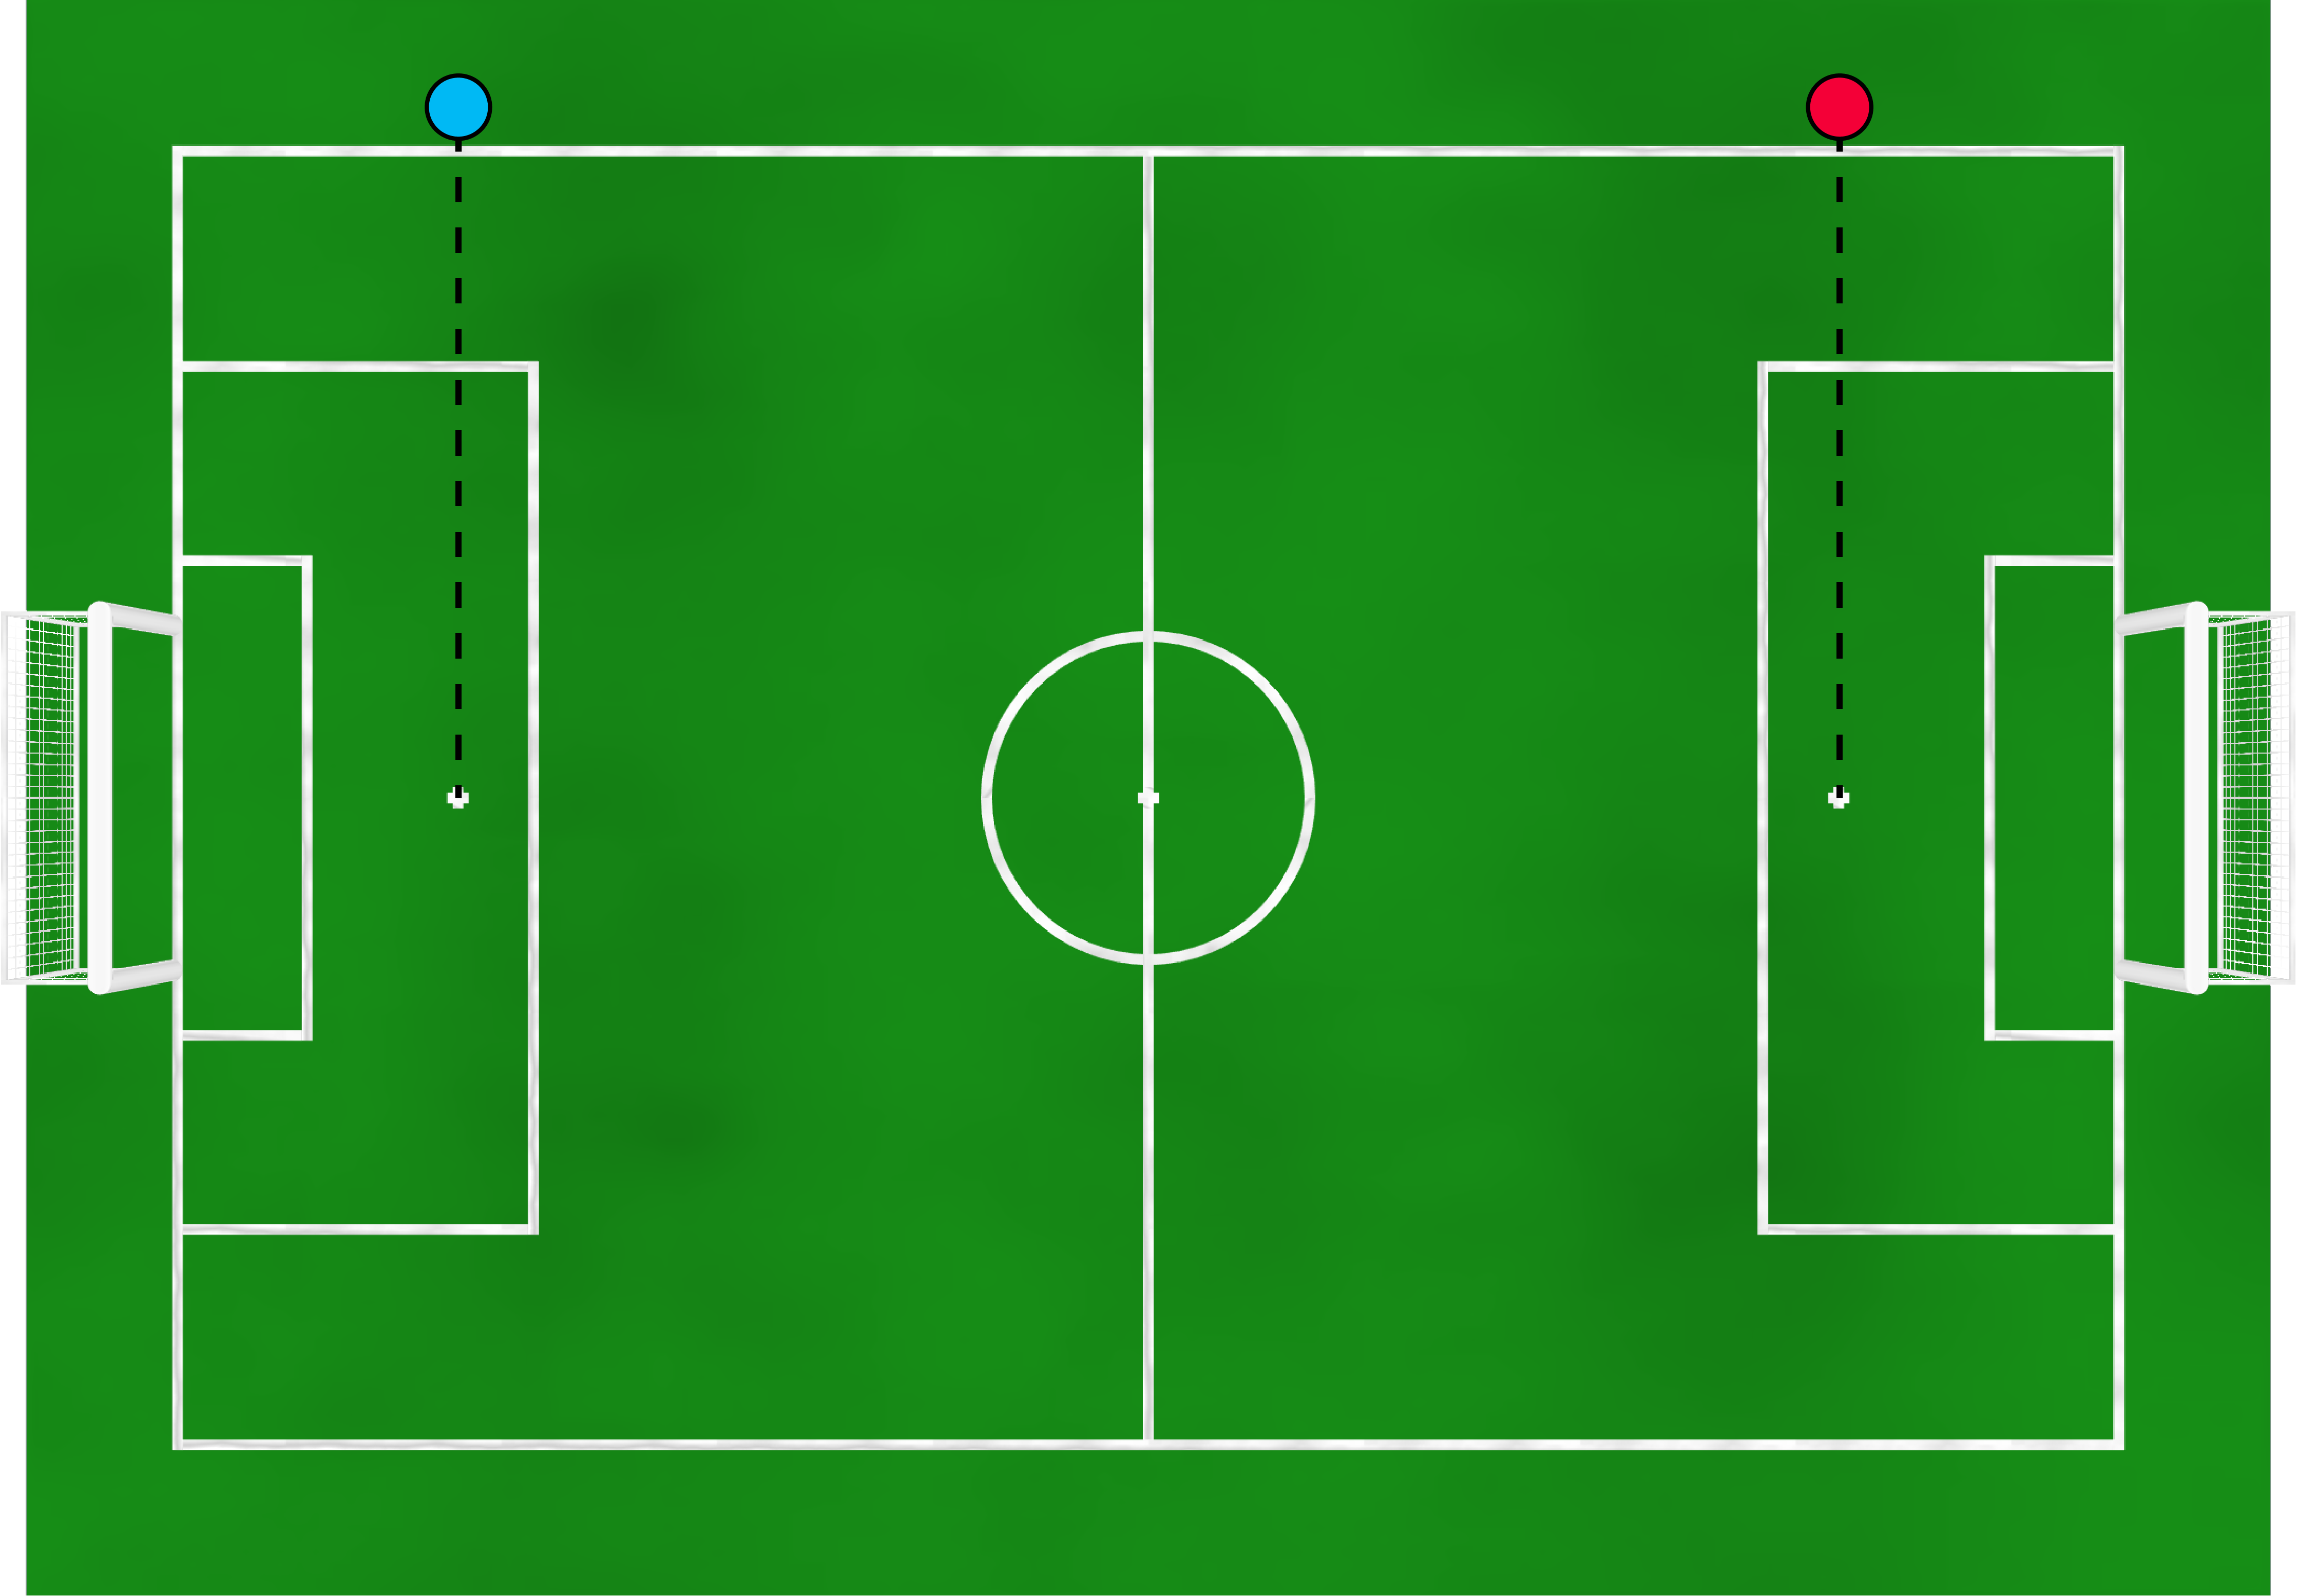
\includegraphics[width=\columnwidth]{figs/penalty_re-entry_points_2020.png}}
	\caption{For robots coming back from a standard removal penalty, re-entry points  are inline with the penalty spot in their own half, on the sideline on the side away from the ball.}
	\label{fig:penalty_re-entry_points}
\end{figure}

When the robot is on the field again, the operator of the GameController will send the \emph{playing} signal to it.

\subsubsection{Forbidden Actions}

The following actions are forbidden, but not treated as penalties.
Each forbidden action specifies the actions to be taken by the referees.

\subparagraph{Manual Interaction by Team Members}

Manual interaction with the robots, either directly or via some communications mechanism, is not permitted.

\subparagraph{Locomotion Type}
\label{sec:locomotion_type}

Robots should clearly demonstrate bipedal walking similar to human walking. Other types of locomotion involving other parts than feet (crawling etc.) are strictly forbidden.
The head referee decides whether a robot's locomotion is appropriate. Robots using inappropriate locomotion types will be removed via ``Request for Pick-up'' until they are able to show appropriate locomotion.

\subparagraph{Damage to the Field}
\label{sec:damage}

A robot that damages the field, or poses a threat to spectator safety, will be removed from the field for the remainder of the \cbw{competition}.

\cbp{\subparagraph{Damage to the Robot}
\label{sec:damage_robot}

The head referee decides whether a robot excessively damages itself and should remove it from the field via ``Request for Pick-up''. 
All referees are allowed to prevent robots from crashing to the ground by catching them beforehand and then laying them down gently. Robots are not allowed to dive for the ball on purpose (\cf section \ref{sec:fallenrobots}).}

\subsubsection{Illegal Positioning}
\label{sec:illegal_positioning}

A robot penalized under illegal position has the ``Illegal Position'' penalty applied. Illegally positioned robots are subject to the standard removal penalty (\cf Section~\ref{sec:removal_penalty}).
The head referee will call ``Illegal Position  \textless robot\textgreater''.

For simplicity, Illegal Positioning penalties during the \textit{Set} state (for kick-off) do not count towards the incremental penalty count\footnote{Historically, the Illegal Positioning penalty only occurred during a kick-off, and other illegal actions were termed Illegal Defender. Illegal Positioning \& Defender have been merged, but the penalty count left unchanged.}.

Refer to Section~\ref{sec:inside_outside} for the definition of \textit{inside/outside} of a region of the field.

``Illegal Position'' shall be imposed if a robot is not inside its own half at the time the Set state starts. It will then be penalized and removed for 15 seconds. The centre line does not count as part of the own half for this penalty, \cbw{nor does the area inside the goal!}

\subsubsection{Motion in Set}
\label{sec:motion_in_set}

Robots may not exit the Set state until either the referee's whistle is detected or a GameController Playing signal has been received.
The head referee will call ``Motion in Set \textless robot\textgreater''.
The offending robot is penalized \textit{in-place} on the field. It will then be unable to move until it receives the GameController Playing signal. Motion in Set penalties do not follow the standard removal procedure, and hence do not count towards the incremental penalty count.

\subsubsection{Fallen or Inactive Robots}
\label{sec:fallenrobots}

If a robot falls during the game, it should start executing a getup action within 5 seconds. If it does not commence a get up action within 5 seconds, it will be penalized and removed for \StandardPenaltyTime.
A robot which is unable to autonomously stand up within 20 seconds after a fall \cbw{and be at least 10 seconds upright} will be penalized and removed for \StandardPenaltyTime. 
In both cases, the head referee will call ``Fallen Robot  \textless robot\textgreater''.

\cbw{\textbf{No robot}} is permitted to `dive' (that is deliberately fall in a way that might cause its torso, arms or hands) to intercept the ball. The robots should be programmed to attempt to remain upright -- that is, supported by its feet.

A robot that has ceased activity for 10 seconds or has turned off will be removed and penalized for 45 seconds.
The head referee will call ``Inactive Robot  \textless robot\textgreater''.
A robot is active if it performs at least one of the following:
\begin{enumerate}
	\item The robot walks in any direction, or turns.
	\item The robot searches for the ball, or is looking at the ball.
\end{enumerate}

Fallen/Inactive Robot penalties do not follow the standard removal procedure, and hence do not count towards the incremental penalty count.

\subparagraph{Note:} The intention of this rule is not to penalize robots simply for being stationary -- provided they are not `asleep' and have not `crashed'.

\subsubsection{Player Stance}
\label{sec:player_stance}
\cbw{In order to intercept kicked balls the robots are} allowed to go into a wide stance as long as they come back to a normal stance within 5 seconds \cbw{and do not excessively damage the robots}\footnote{\cbw{``excessively'' is decided by the head referee in order to limit damages to robots}}. \\
Robots are not allowed to stay in a stance that is wider than the width of the robot's shoulders for more than 5 seconds. Staying in a wide stance for longer than 5 seconds will result in the standard removal penalty. \\
If the robot has fallen down, it must start getting up within 5 seconds. 

\subsubsection{Playing with Arms/Hands}
\label{sec:hand_ball}

Playing with arms/hands occurs when a field player moves its arms/hands to touch the ball (except during a fall or get-up). A robot playing with arms/hands will be subject to the standard removal penalty and the ball will be replaced at the point where it contacted the arms/hands of the offending robot. If an own goal is scored as a result, the goal should count and the player should not be penalized.
%TODO: Remove the own goal thing?

Accidental playing with arms/hands when a robot falls or executes a get-up routine will not be penalized. 
If the ball goes out of play in this case, normal kick-in rules will apply (\cf Section~\ref{sec:kick_in}). 
Goals resulting from a ball contact with the arms/hands during a fall or get-up do not count and result in a \cbw{kick-in (\cf Section~\ref{sec:kick_in})} as if the ball went over the goal line next to the goal.

\subsubsection{Leaving the Field}
\label{sec:leaving_field}

A robot that intends to leave the \TotalWidth $\times$ \cbw{3.7~m\xspace} carpeted area of its \cbw{\textbf{own half}} will be subject to the standard removal penalty (\cf Section~\ref{sec:removal_penalty})!

\cbp{A touching/exceeding of the centre/halfway line also leads to this standard removal penalty.}

The head referee will call ``Leaving the Field \textless robot\textgreater''.

Additionally, a robot will also be subject to the standard removal penalty when:
\begin{itemize}
	\item the robot walks into the goal posts or \cbw{into the goal area} for more than 5 seconds, this includes robots that are stuck on the goal posts and unable to free themselves
	\item the robot's finger become entangled in the net (without any time constraint).
\end{itemize}

\subsection{Judgment}
\label{sec:judgment}
The referees are the only persons permitted on the carpeted area (\ie the field and the border area).

\cbp{The local team of an arena has to provide the referees. The number of referees depends on local regulations and can be reduced to a head referee and an operator of the GameController.}

\cbp{All referees are allowed to prevent robots from crashing to the ground by catching them beforehand and then laying them down gently!}

\subsubsection{Head Referee}
\label{sec:head_referee}

The head referee is in charge of the game. Any decision of the head referee is valid. The head referee's decision is final and can not be changed afterwards, even by video proof. There is no discussion about decisions during the game, neither between the assistant referees and the head referee, nor between the audience/spectators or the teams and the head referee.

\cbp{The head referee also decides whether a robot excessively damages itself and should be removed from the field (\cf Section~\ref{sec:damage})}.

The head referee announces decisions by a clear loud call, and (as required) whistle sound.
The whistle, or where there is no whistle the first verbal word of the referees calls, defines the point in time at which the decision is made.
The referees should make efforts to use consistent and clear calls, and it is preferable for referees to use the calls as specified in these rules\footnote{The calls specified in these rules are detailed in English. With the agreement of the teams, the referees may use suitable calls in any language. The exception to this are technical challenge(s) that depends on the calls as specified.}.
The intention of specifying the referee calls is for clarity and consistency across games.

Where a whistle is required, the head referee first whistles and then announces the reason for the whistle.
The head referee may choose to use any normal sports whistle.
Each whistle sound should be short and not too loud.
The head referee must \textit{only} sound the whistle in circumstances described in these rules.
There are three circumstances when the whistle is sounded, Kick-off~(\cf Section~\ref{sec:kick-off}), a goal~(\cf Section~\ref{sec:goal}), and ending a half of gameplay~(\cf Section~\ref{sec:game_struct}).

The head referee should avoid handling the ball (except for placing \cbw{the balls} for a kick-off), and avoid handling the robots.
Their duty is to monitor and adjudicate the game.
The head referee should only handle robots and the ball if absolutely necessary to expedite gameplay or removal of penalized robots, where the assistant referees are otherwise occupied, are too far away \cbw{or had to be dropped due to local regulations.}

\subsubsection{Assistant Referees}
\label{sec:assist_referee}
The, \cbw{in the ideal case}, two assistant referees handle the robots and the balls. They start the robots if they are not using the GameController, they move the robots, if a manual placement is needed, they take the robots out when they are penalized, and they put the robots in again. An assistant referee will also replace the ball when it goes off the field or becomes stuck between a players feet.

\cbp{If a team requests to pick up a robot, an assistant referee will pick it up and put it on the sideline. Also the assistant, on behalf of the teams, can do hardware changes to robots on the sideline, \ie reboot it or change and secure the battery.}

The assistant referees can \textit{indicate} violations against the rules committed by robots to the head referee, so that the head referee can decide whether to penalize a certain robot or not. Assistant referees should only enter the field to execute a decision made by the main referee \cbw{or to catch a falling robot}.

\subsubsection{Operator of the GameController}
\label{sec:gameControllerOp}
The operator of the GameController sits at a PC outside the playing area.
As with the head referee, the operator should make efforts to use consistent and clear calls.
They will signal any change in the game state to the robots via the wireless as they are announced by the head referee.
Note that for both kick-offs and goals, the moment of whistling is determining, not the verbal announcement of the head referee.
The operator will also inform the assistant referees when a timed penalty is over and a robot has to be placed back on the field.
They should announce when the ball is in play on kick-off by stating ``Ball Free'', if the \KickOffBallFreeTime time period has elapsed in the playing state.
They are also responsible for keeping the time of each half (\ie, they stop the clock after a global game stuck, and continues it at the kick-off).
They should count aloud the remaining seconds in a half once the time remaining is 5 seconds or less.
Finally, they should repeat the calls of the head referee to make sure it was heard correctly.

\subsubsection{Referees During the Match}

The head referee and the assistant referees should wear clothing and socks \emph{of black or dark blue colour} (blue jeans are acceptable) and avoid reserved colours for the ball, the goals, and player markings in their clothing. They may enter the field in particular situations, \eg, to remove a robot when applying a penalty \cbw{or to catch a falling robot}. They should avoid interfering with the robots as much as possible.

\subsubsection{A Remark on Artificial Landmarks}
\label{sec:judgment:landmarks}

The head referee may decide at any point before or during a game to relocate any objects around the field, or direct persons to another position around the field.

The intent of using same-coloured goals is to remove artificial landmarks.
Robots should be able to localize with the SPL field and its ``normal'' surroundings.
Introducing new team-specific artificial landmarks is against the spirit and intention of the league's progress.
The application of this rule needs to be well considered and should be reserved for situations which seem constructed by one team or another, but will ultimately be the head referee's decision alone.

\newpage

\subsection{Technical Field Drawings}
\label{apx:technical-drawing}
\centerline{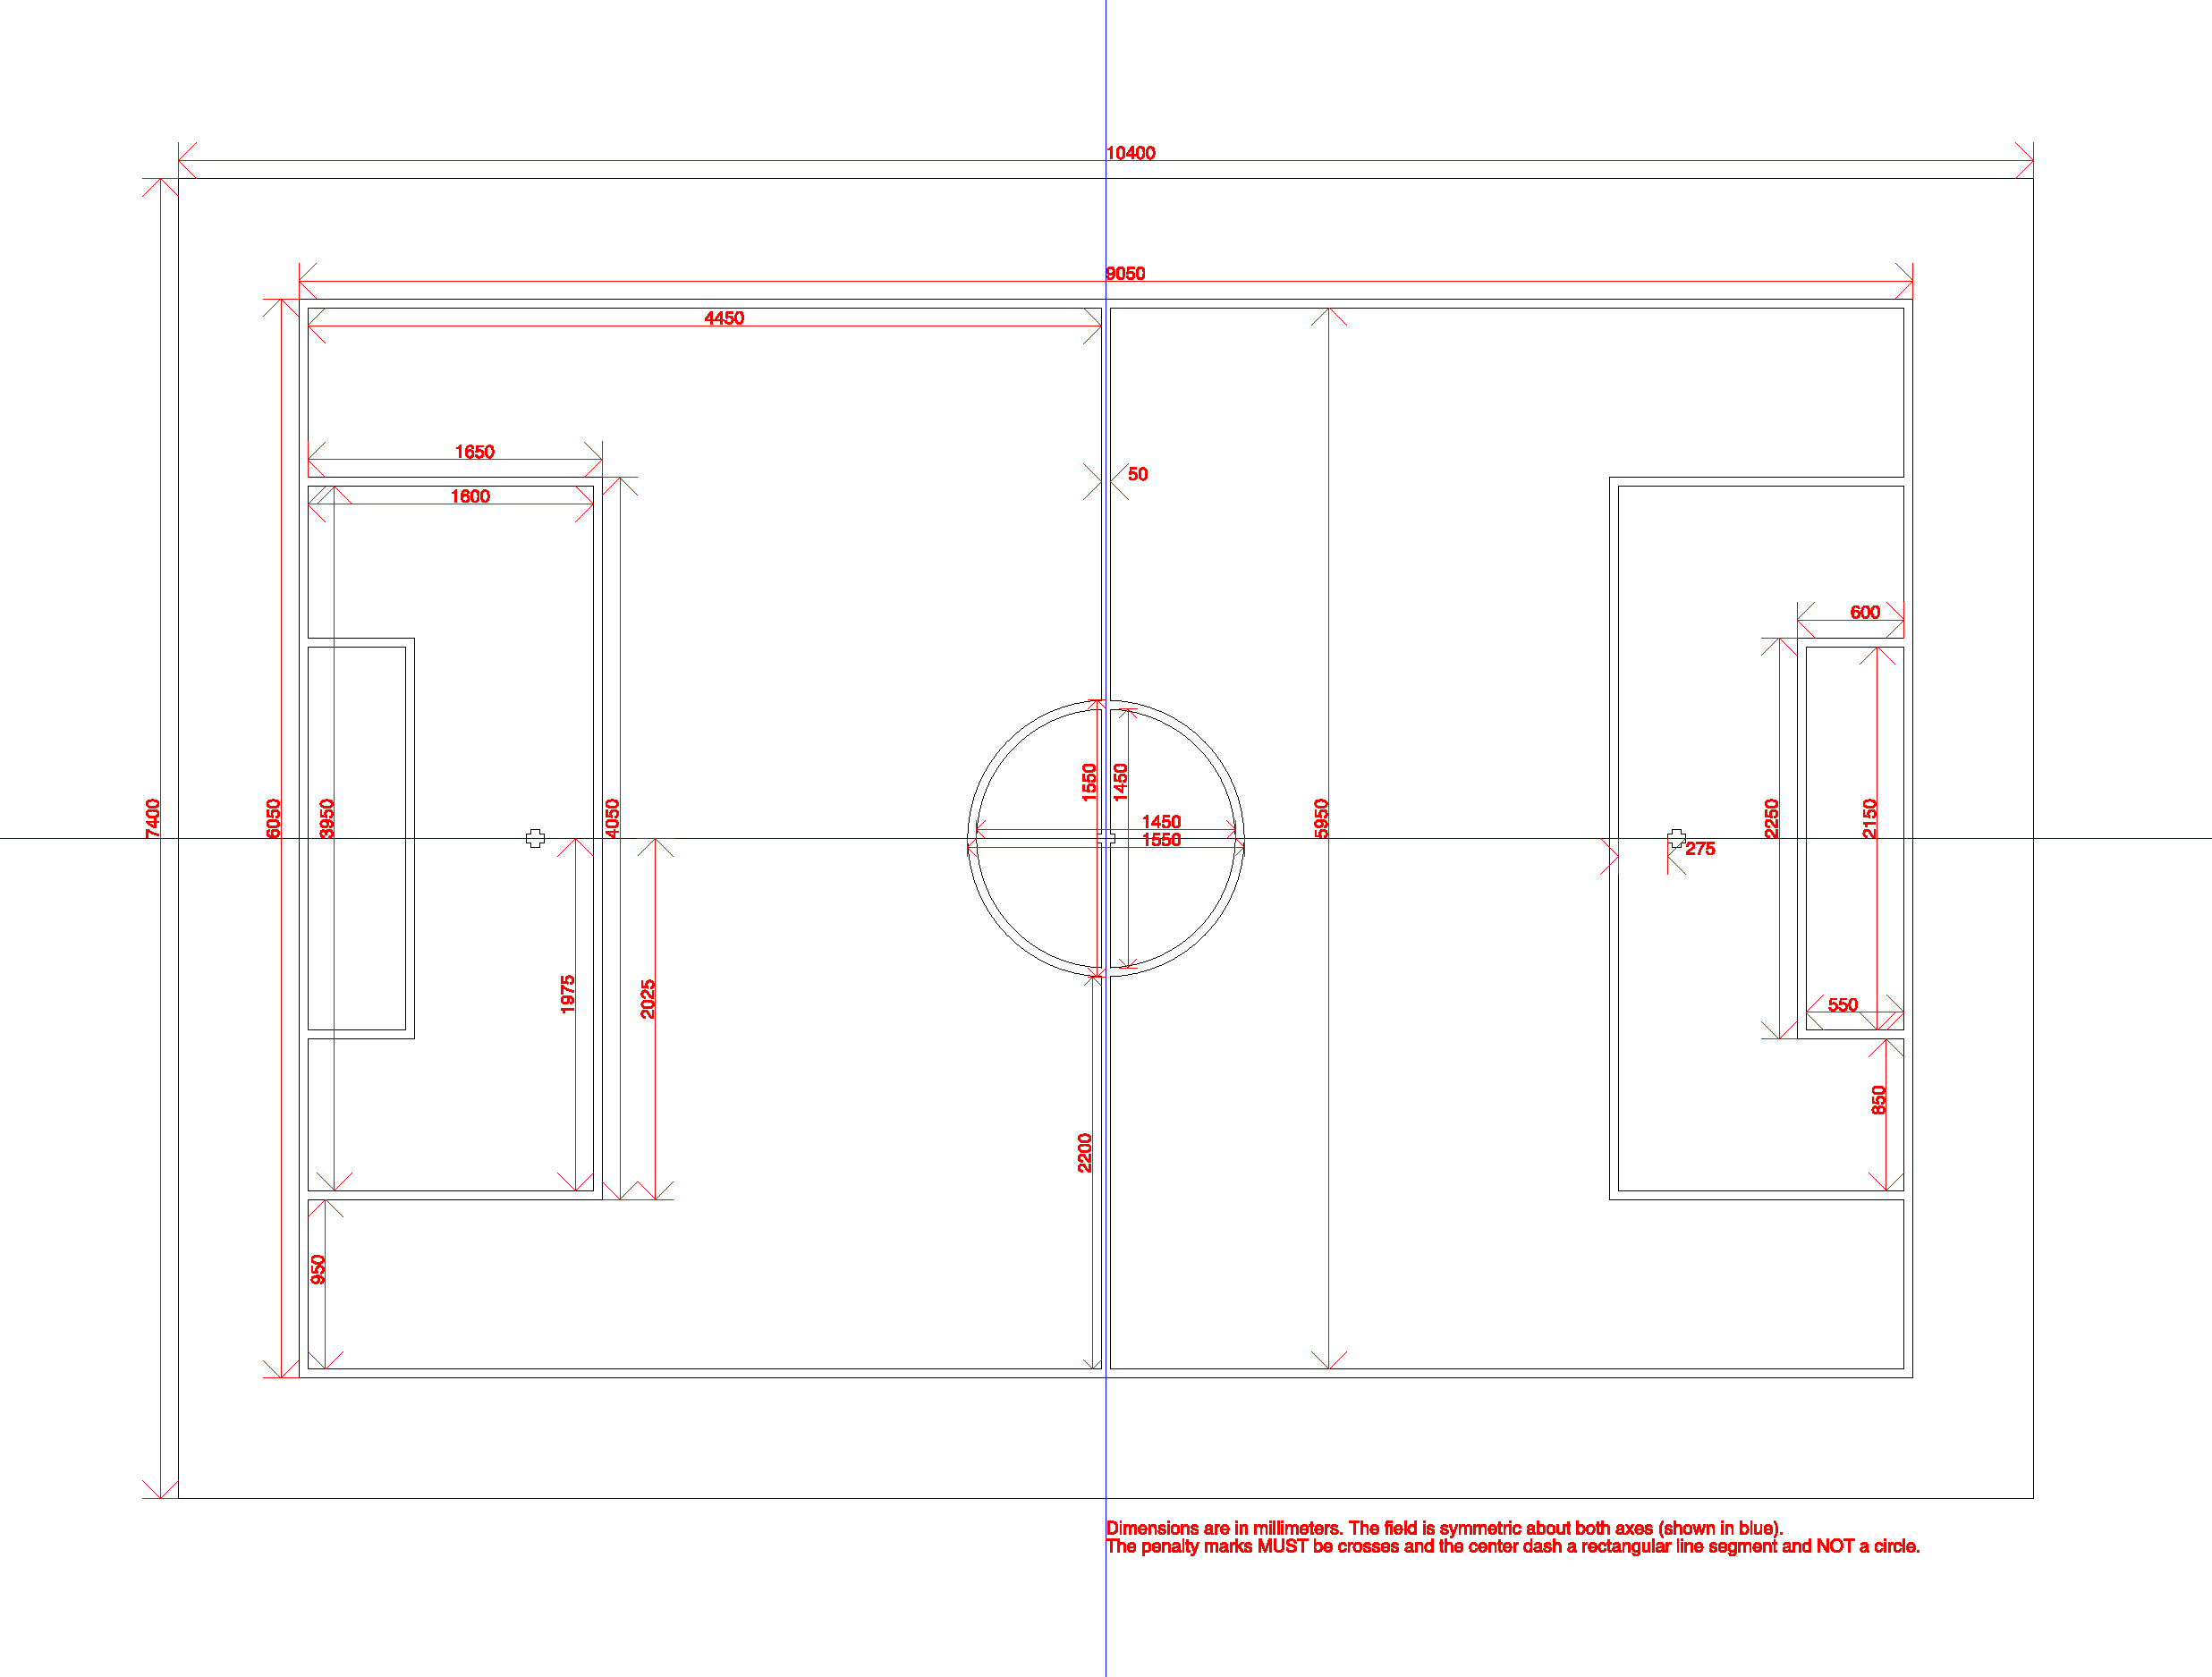
\includegraphics[angle=90,origin=c,width=\columnwidth]{figs/fieldDimensions2020_technical.pdf}}

\clearpage
\centerline{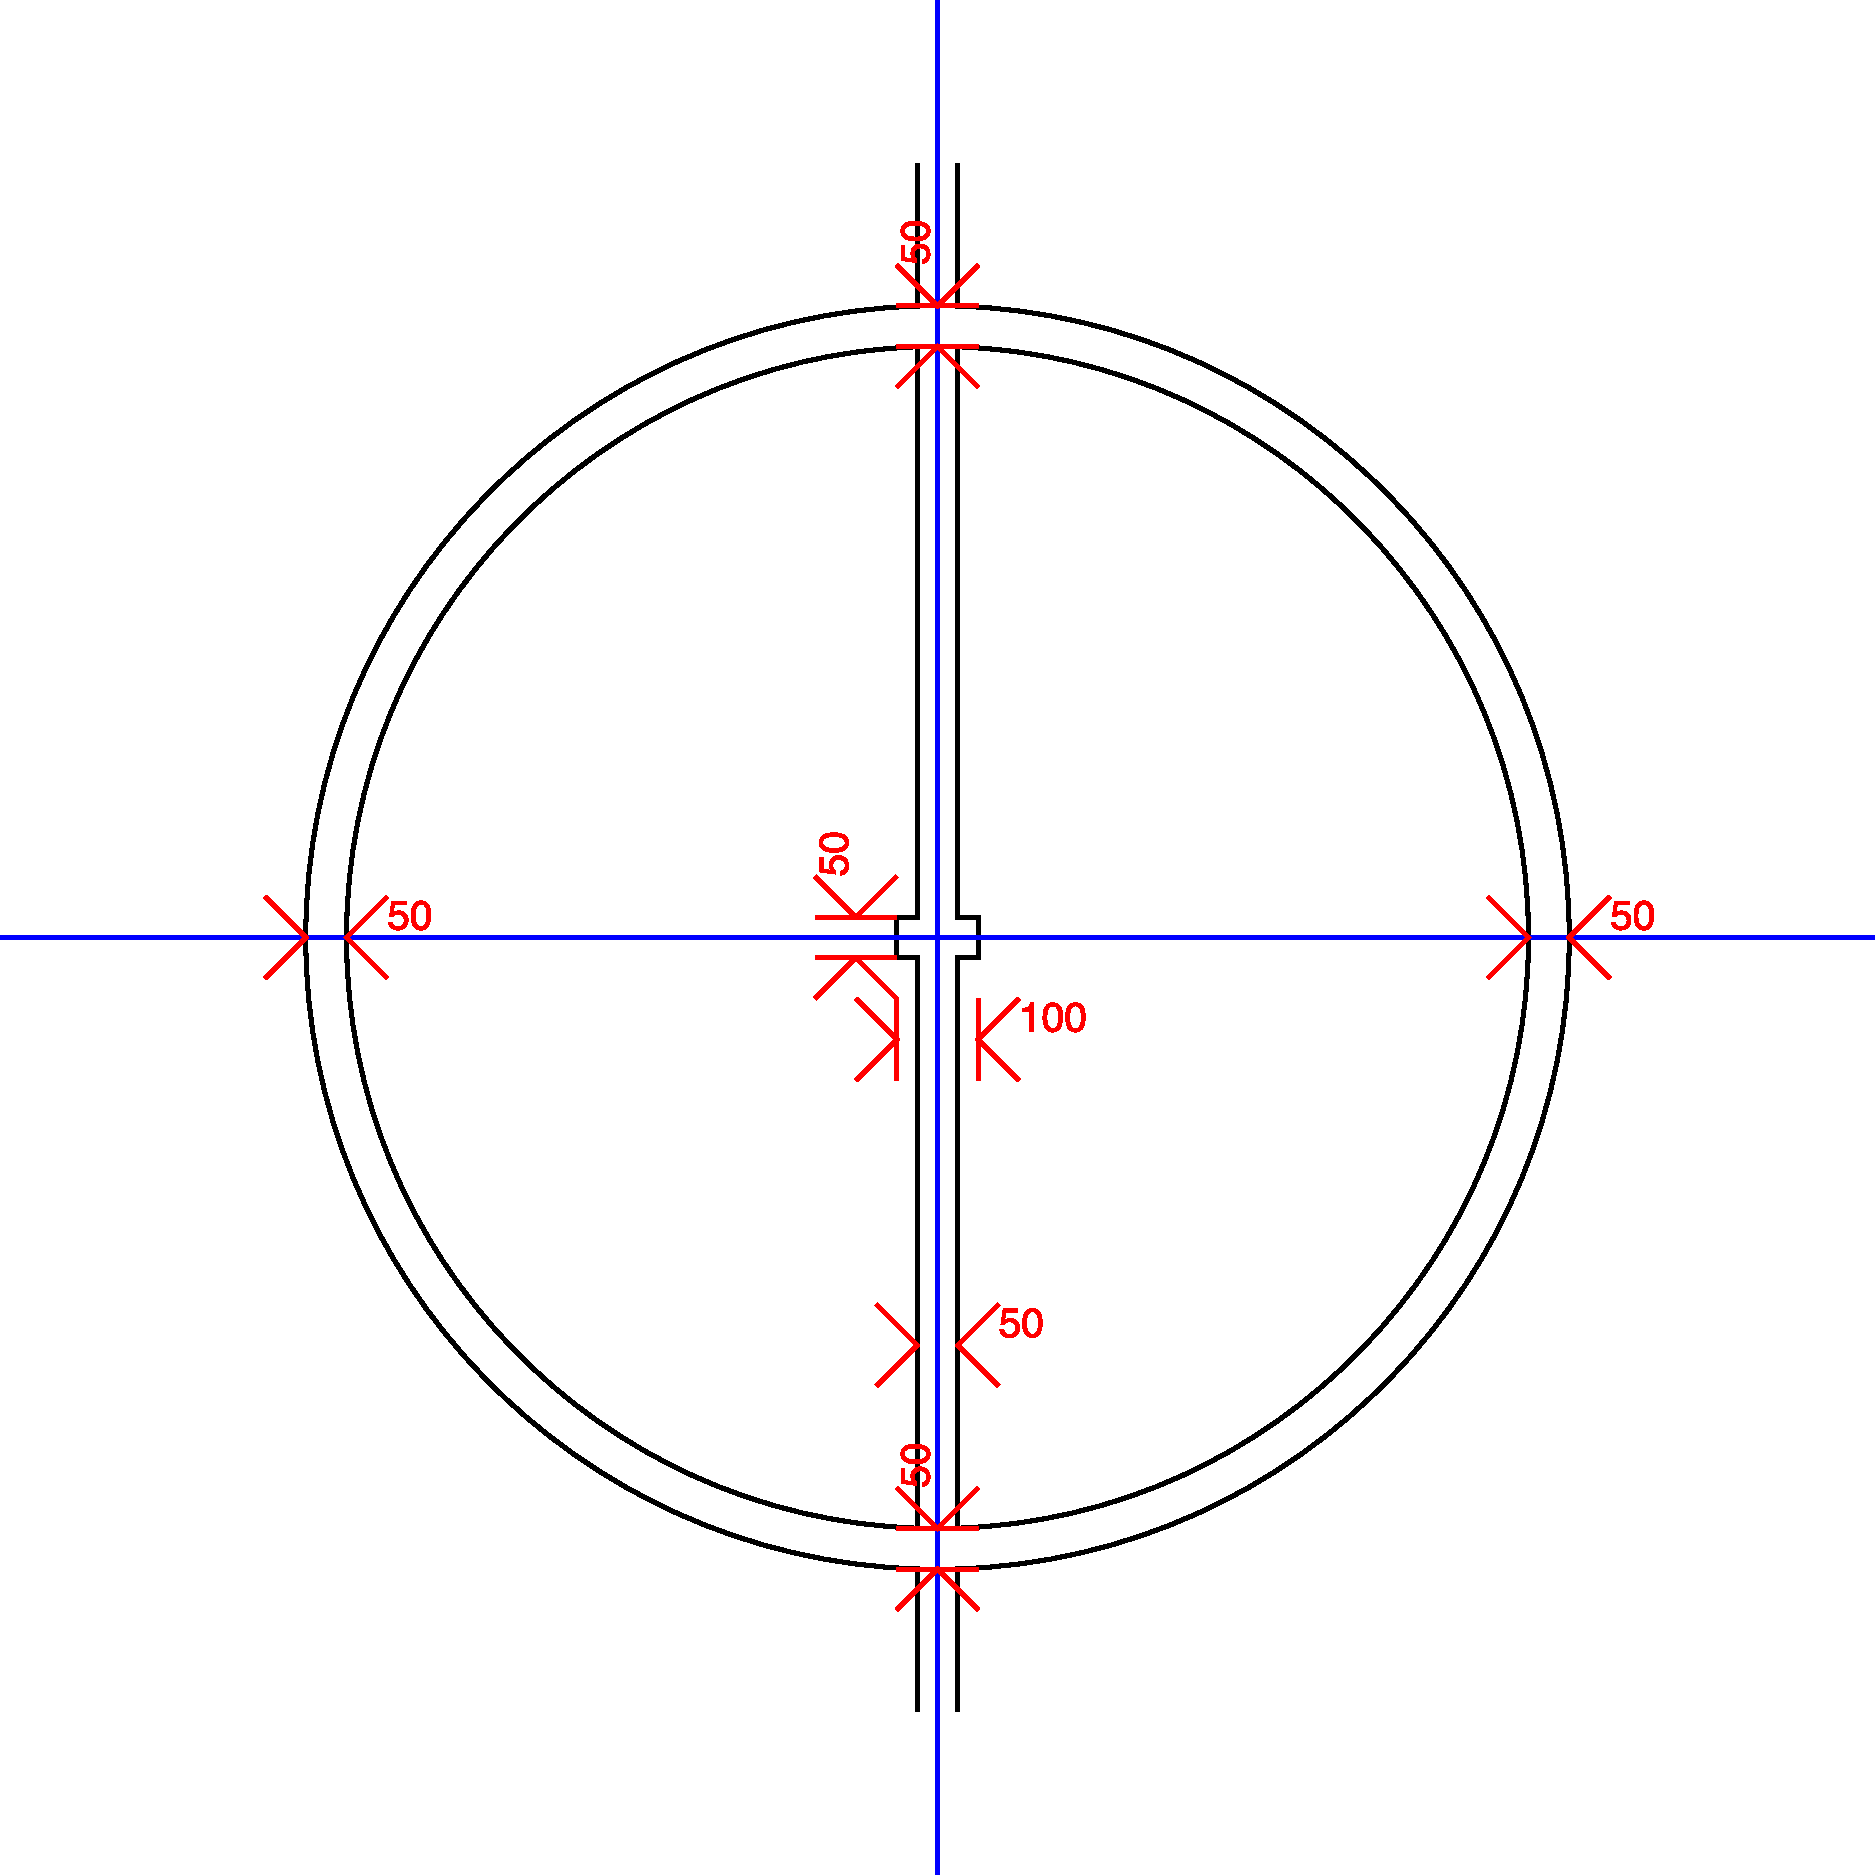
\includegraphics[angle=90,origin=c,width=0.5\columnwidth]{figs/fieldDimensions2020_technical_cc.pdf}}

\centerline{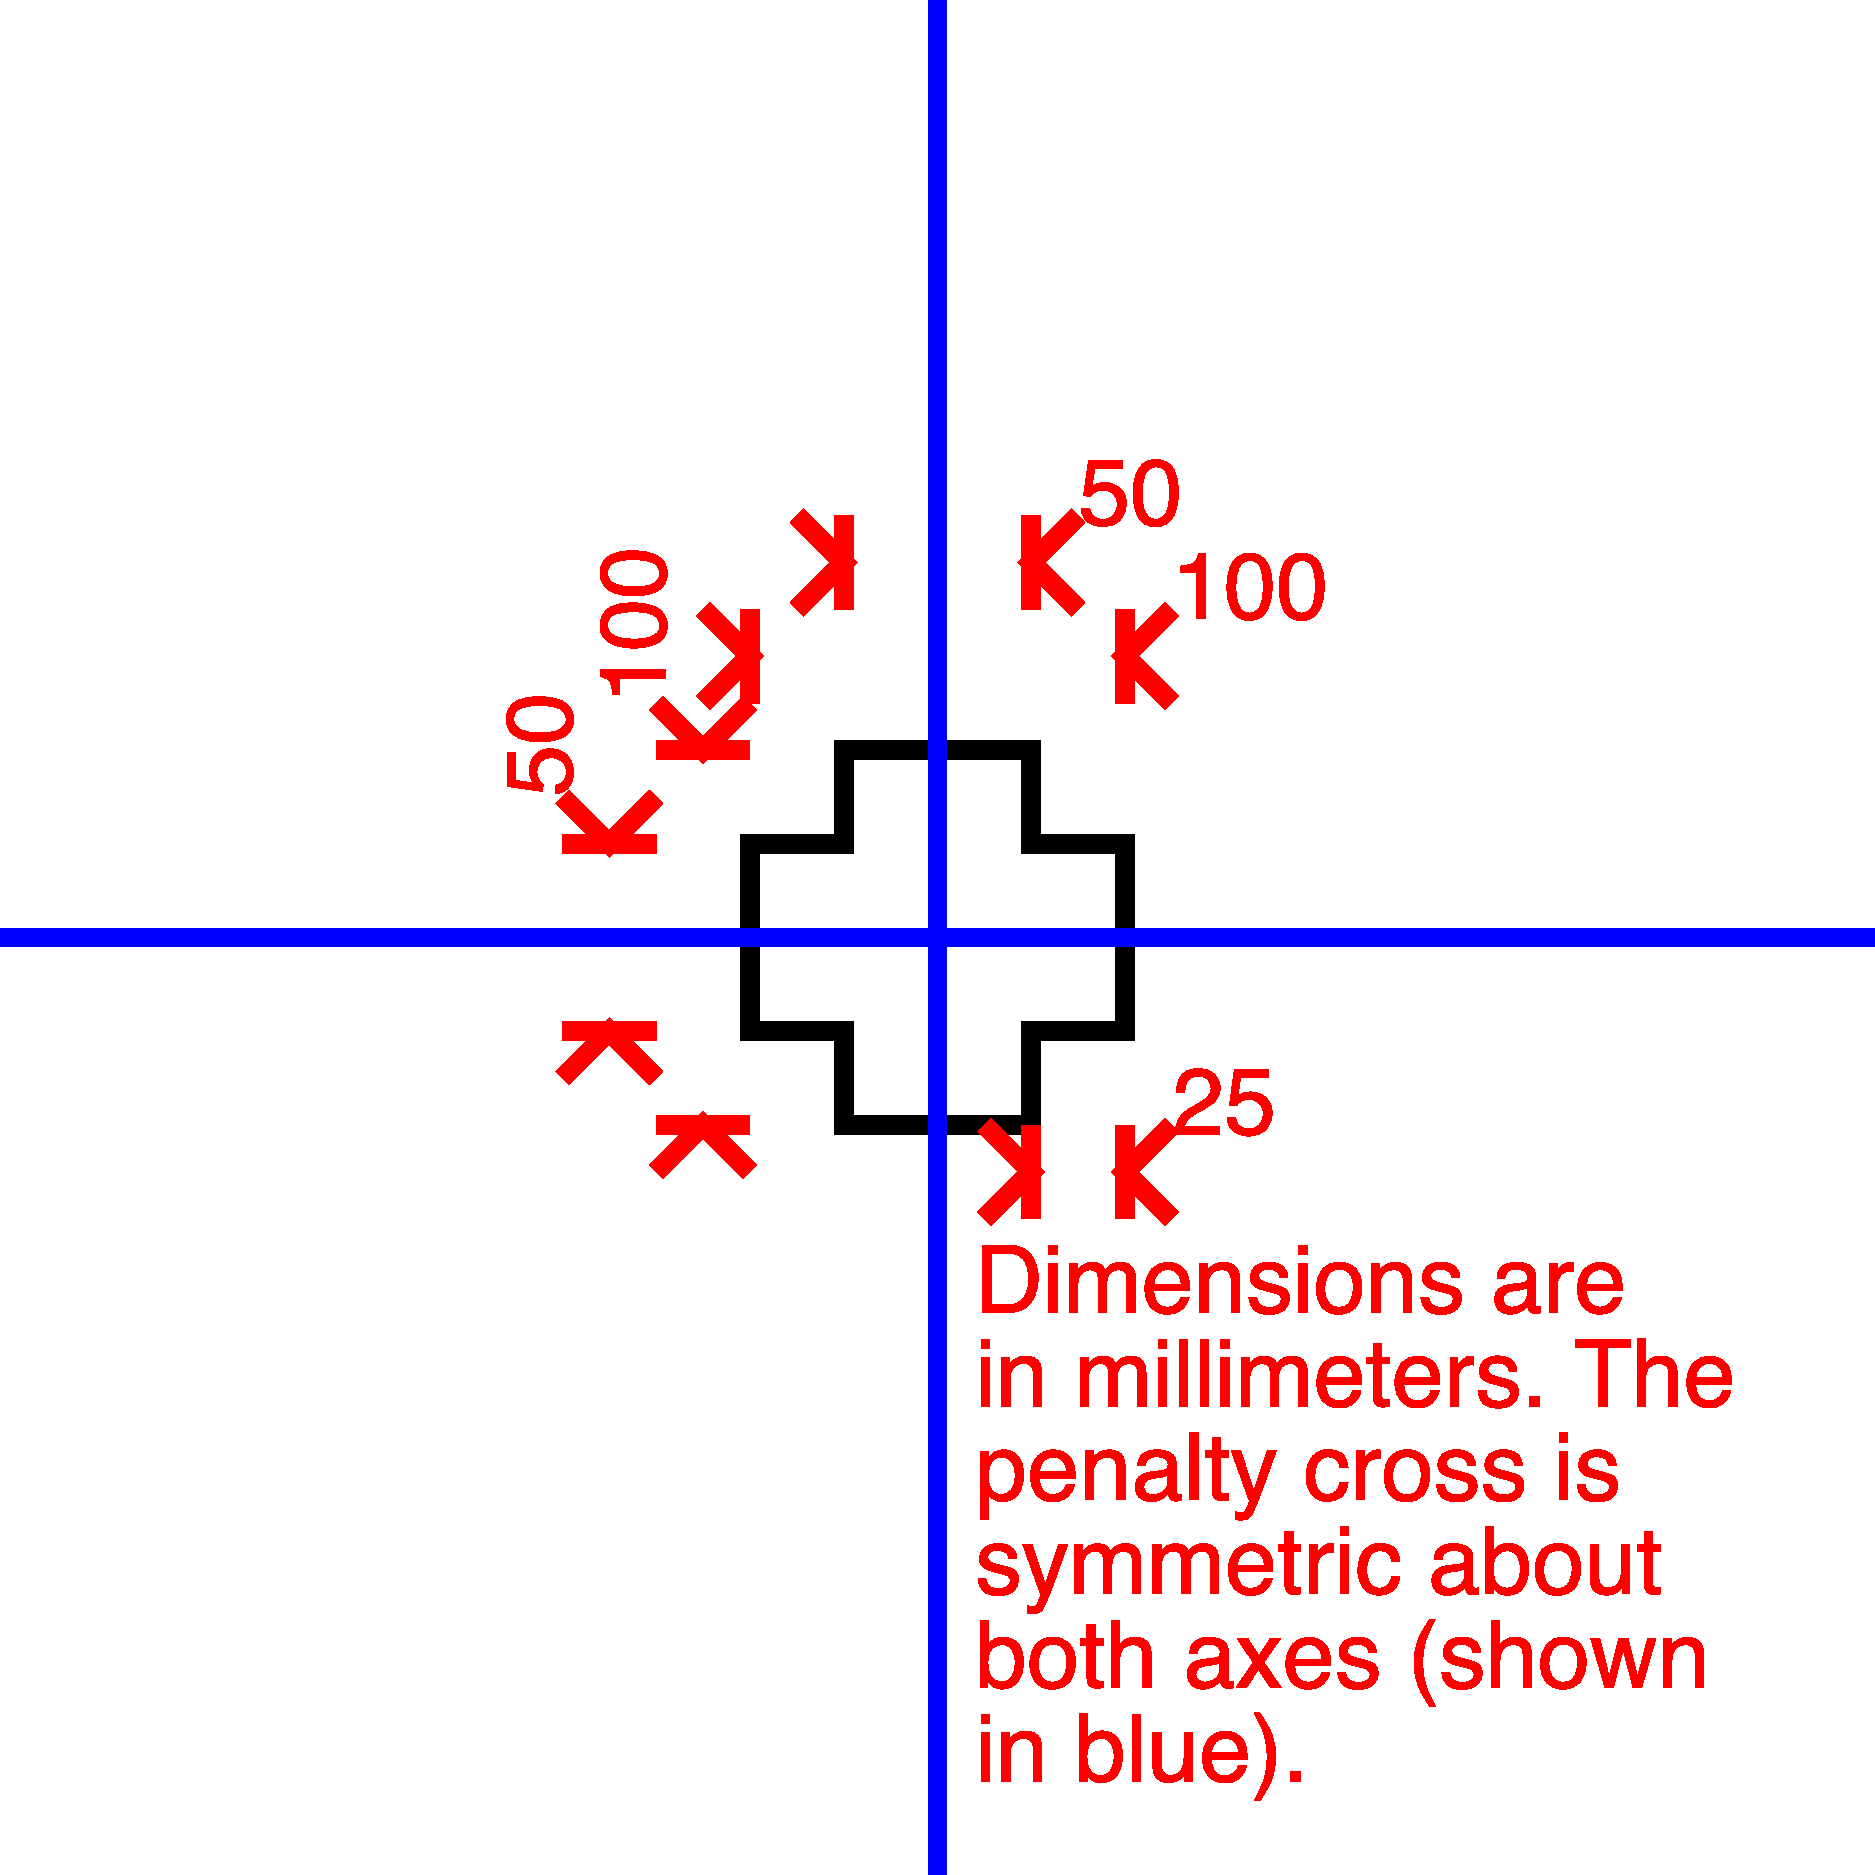
\includegraphics[origin=c,width=0.5\columnwidth]{figs/fieldDimensions2020_technical_pc.pdf}}
